% Options for packages loaded elsewhere
\PassOptionsToPackage{unicode}{hyperref}
\PassOptionsToPackage{hyphens}{url}
\PassOptionsToPackage{dvipsnames,svgnames,x11names}{xcolor}
%
\documentclass[
]{interact}

\usepackage{amsmath,amssymb}
\usepackage{iftex}
\ifPDFTeX
  \usepackage[T1]{fontenc}
  \usepackage[utf8]{inputenc}
  \usepackage{textcomp} % provide euro and other symbols
\else % if luatex or xetex
  \usepackage{unicode-math}
  \defaultfontfeatures{Scale=MatchLowercase}
  \defaultfontfeatures[\rmfamily]{Ligatures=TeX,Scale=1}
\fi
\usepackage{lmodern}
\ifPDFTeX\else  
    % xetex/luatex font selection
\fi
% Use upquote if available, for straight quotes in verbatim environments
\IfFileExists{upquote.sty}{\usepackage{upquote}}{}
\IfFileExists{microtype.sty}{% use microtype if available
  \usepackage[]{microtype}
  \UseMicrotypeSet[protrusion]{basicmath} % disable protrusion for tt fonts
}{}
\makeatletter
\@ifundefined{KOMAClassName}{% if non-KOMA class
  \IfFileExists{parskip.sty}{%
    \usepackage{parskip}
  }{% else
    \setlength{\parindent}{0pt}
    \setlength{\parskip}{6pt plus 2pt minus 1pt}}
}{% if KOMA class
  \KOMAoptions{parskip=half}}
\makeatother
\usepackage{xcolor}
\setlength{\emergencystretch}{3em} % prevent overfull lines
\setcounter{secnumdepth}{5}
% Make \paragraph and \subparagraph free-standing
\makeatletter
\ifx\paragraph\undefined\else
  \let\oldparagraph\paragraph
  \renewcommand{\paragraph}{
    \@ifstar
      \xxxParagraphStar
      \xxxParagraphNoStar
  }
  \newcommand{\xxxParagraphStar}[1]{\oldparagraph*{#1}\mbox{}}
  \newcommand{\xxxParagraphNoStar}[1]{\oldparagraph{#1}\mbox{}}
\fi
\ifx\subparagraph\undefined\else
  \let\oldsubparagraph\subparagraph
  \renewcommand{\subparagraph}{
    \@ifstar
      \xxxSubParagraphStar
      \xxxSubParagraphNoStar
  }
  \newcommand{\xxxSubParagraphStar}[1]{\oldsubparagraph*{#1}\mbox{}}
  \newcommand{\xxxSubParagraphNoStar}[1]{\oldsubparagraph{#1}\mbox{}}
\fi
\makeatother

\usepackage{color}
\usepackage{fancyvrb}
\newcommand{\VerbBar}{|}
\newcommand{\VERB}{\Verb[commandchars=\\\{\}]}
\DefineVerbatimEnvironment{Highlighting}{Verbatim}{commandchars=\\\{\}}
% Add ',fontsize=\small' for more characters per line
\usepackage{framed}
\definecolor{shadecolor}{RGB}{241,243,245}
\newenvironment{Shaded}{\begin{snugshade}}{\end{snugshade}}
\newcommand{\AlertTok}[1]{\textcolor[rgb]{0.68,0.00,0.00}{#1}}
\newcommand{\AnnotationTok}[1]{\textcolor[rgb]{0.37,0.37,0.37}{#1}}
\newcommand{\AttributeTok}[1]{\textcolor[rgb]{0.40,0.45,0.13}{#1}}
\newcommand{\BaseNTok}[1]{\textcolor[rgb]{0.68,0.00,0.00}{#1}}
\newcommand{\BuiltInTok}[1]{\textcolor[rgb]{0.00,0.23,0.31}{#1}}
\newcommand{\CharTok}[1]{\textcolor[rgb]{0.13,0.47,0.30}{#1}}
\newcommand{\CommentTok}[1]{\textcolor[rgb]{0.37,0.37,0.37}{#1}}
\newcommand{\CommentVarTok}[1]{\textcolor[rgb]{0.37,0.37,0.37}{\textit{#1}}}
\newcommand{\ConstantTok}[1]{\textcolor[rgb]{0.56,0.35,0.01}{#1}}
\newcommand{\ControlFlowTok}[1]{\textcolor[rgb]{0.00,0.23,0.31}{\textbf{#1}}}
\newcommand{\DataTypeTok}[1]{\textcolor[rgb]{0.68,0.00,0.00}{#1}}
\newcommand{\DecValTok}[1]{\textcolor[rgb]{0.68,0.00,0.00}{#1}}
\newcommand{\DocumentationTok}[1]{\textcolor[rgb]{0.37,0.37,0.37}{\textit{#1}}}
\newcommand{\ErrorTok}[1]{\textcolor[rgb]{0.68,0.00,0.00}{#1}}
\newcommand{\ExtensionTok}[1]{\textcolor[rgb]{0.00,0.23,0.31}{#1}}
\newcommand{\FloatTok}[1]{\textcolor[rgb]{0.68,0.00,0.00}{#1}}
\newcommand{\FunctionTok}[1]{\textcolor[rgb]{0.28,0.35,0.67}{#1}}
\newcommand{\ImportTok}[1]{\textcolor[rgb]{0.00,0.46,0.62}{#1}}
\newcommand{\InformationTok}[1]{\textcolor[rgb]{0.37,0.37,0.37}{#1}}
\newcommand{\KeywordTok}[1]{\textcolor[rgb]{0.00,0.23,0.31}{\textbf{#1}}}
\newcommand{\NormalTok}[1]{\textcolor[rgb]{0.00,0.23,0.31}{#1}}
\newcommand{\OperatorTok}[1]{\textcolor[rgb]{0.37,0.37,0.37}{#1}}
\newcommand{\OtherTok}[1]{\textcolor[rgb]{0.00,0.23,0.31}{#1}}
\newcommand{\PreprocessorTok}[1]{\textcolor[rgb]{0.68,0.00,0.00}{#1}}
\newcommand{\RegionMarkerTok}[1]{\textcolor[rgb]{0.00,0.23,0.31}{#1}}
\newcommand{\SpecialCharTok}[1]{\textcolor[rgb]{0.37,0.37,0.37}{#1}}
\newcommand{\SpecialStringTok}[1]{\textcolor[rgb]{0.13,0.47,0.30}{#1}}
\newcommand{\StringTok}[1]{\textcolor[rgb]{0.13,0.47,0.30}{#1}}
\newcommand{\VariableTok}[1]{\textcolor[rgb]{0.07,0.07,0.07}{#1}}
\newcommand{\VerbatimStringTok}[1]{\textcolor[rgb]{0.13,0.47,0.30}{#1}}
\newcommand{\WarningTok}[1]{\textcolor[rgb]{0.37,0.37,0.37}{\textit{#1}}}

\providecommand{\tightlist}{%
  \setlength{\itemsep}{0pt}\setlength{\parskip}{0pt}}\usepackage{longtable,booktabs,array}
\usepackage{calc} % for calculating minipage widths
% Correct order of tables after \paragraph or \subparagraph
\usepackage{etoolbox}
\makeatletter
\patchcmd\longtable{\par}{\if@noskipsec\mbox{}\fi\par}{}{}
\makeatother
% Allow footnotes in longtable head/foot
\IfFileExists{footnotehyper.sty}{\usepackage{footnotehyper}}{\usepackage{footnote}}
\makesavenoteenv{longtable}
\usepackage{graphicx}
\makeatletter
\newsavebox\pandoc@box
\newcommand*\pandocbounded[1]{% scales image to fit in text height/width
  \sbox\pandoc@box{#1}%
  \Gscale@div\@tempa{\textheight}{\dimexpr\ht\pandoc@box+\dp\pandoc@box\relax}%
  \Gscale@div\@tempb{\linewidth}{\wd\pandoc@box}%
  \ifdim\@tempb\p@<\@tempa\p@\let\@tempa\@tempb\fi% select the smaller of both
  \ifdim\@tempa\p@<\p@\scalebox{\@tempa}{\usebox\pandoc@box}%
  \else\usebox{\pandoc@box}%
  \fi%
}
% Set default figure placement to htbp
\def\fps@figure{htbp}
\makeatother
% definitions for citeproc citations
\NewDocumentCommand\citeproctext{}{}
\NewDocumentCommand\citeproc{mm}{%
  \begingroup\def\citeproctext{#2}\cite{#1}\endgroup}
\makeatletter
 % allow citations to break across lines
 \let\@cite@ofmt\@firstofone
 % avoid brackets around text for \cite:
 \def\@biblabel#1{}
 \def\@cite#1#2{{#1\if@tempswa , #2\fi}}
\makeatother
\newlength{\cslhangindent}
\setlength{\cslhangindent}{1.5em}
\newlength{\csllabelwidth}
\setlength{\csllabelwidth}{3em}
\newenvironment{CSLReferences}[2] % #1 hanging-indent, #2 entry-spacing
 {\begin{list}{}{%
  \setlength{\itemindent}{0pt}
  \setlength{\leftmargin}{0pt}
  \setlength{\parsep}{0pt}
  % turn on hanging indent if param 1 is 1
  \ifodd #1
   \setlength{\leftmargin}{\cslhangindent}
   \setlength{\itemindent}{-1\cslhangindent}
  \fi
  % set entry spacing
  \setlength{\itemsep}{#2\baselineskip}}}
 {\end{list}}
\usepackage{calc}
\newcommand{\CSLBlock}[1]{\hfill\break\parbox[t]{\linewidth}{\strut\ignorespaces#1\strut}}
\newcommand{\CSLLeftMargin}[1]{\parbox[t]{\csllabelwidth}{\strut#1\strut}}
\newcommand{\CSLRightInline}[1]{\parbox[t]{\linewidth - \csllabelwidth}{\strut#1\strut}}
\newcommand{\CSLIndent}[1]{\hspace{\cslhangindent}#1}

\usepackage{orcidlink}
\makeatletter
\@ifpackageloaded{caption}{}{\usepackage{caption}}
\AtBeginDocument{%
\ifdefined\contentsname
  \renewcommand*\contentsname{Table of contents}
\else
  \newcommand\contentsname{Table of contents}
\fi
\ifdefined\listfigurename
  \renewcommand*\listfigurename{List of Figures}
\else
  \newcommand\listfigurename{List of Figures}
\fi
\ifdefined\listtablename
  \renewcommand*\listtablename{List of Tables}
\else
  \newcommand\listtablename{List of Tables}
\fi
\ifdefined\figurename
  \renewcommand*\figurename{Figure}
\else
  \newcommand\figurename{Figure}
\fi
\ifdefined\tablename
  \renewcommand*\tablename{Table}
\else
  \newcommand\tablename{Table}
\fi
}
\@ifpackageloaded{float}{}{\usepackage{float}}
\floatstyle{ruled}
\@ifundefined{c@chapter}{\newfloat{codelisting}{h}{lop}}{\newfloat{codelisting}{h}{lop}[chapter]}
\floatname{codelisting}{Listing}
\newcommand*\listoflistings{\listof{codelisting}{List of Listings}}
\makeatother
\makeatletter
\makeatother
\makeatletter
\@ifpackageloaded{caption}{}{\usepackage{caption}}
\@ifpackageloaded{subcaption}{}{\usepackage{subcaption}}
\makeatother

\usepackage{bookmark}

\IfFileExists{xurl.sty}{\usepackage{xurl}}{} % add URL line breaks if available
\urlstyle{same} % disable monospaced font for URLs
\hypersetup{
  pdftitle={mvgam\_uti},
  colorlinks=true,
  linkcolor={blue},
  filecolor={Maroon},
  citecolor={Blue},
  urlcolor={Blue},
  pdfcreator={LaTeX via pandoc}}


\title{mvgam\_uti}
\author{Stefano
Coretta$\textsuperscript{1}$~\orcidlink{0000-0001-9627-5532}, Georges
Sakr$\textsuperscript{1}$}

\thanks{CONTACT: Stefano
Coretta. Email: \href{mailto:s.coretta@ed.ac.uk}{\nolinkurl{s.coretta@ed.ac.uk}}. }
\begin{document}
\captionsetup{labelsep=space}
\maketitle
\textsuperscript{1}  University of Edinburgh,  


\begin{Shaded}
\begin{Highlighting}[]
\FunctionTok{library}\NormalTok{(tidyverse)}
\end{Highlighting}
\end{Shaded}

\begin{verbatim}
-- Attaching core tidyverse packages ------------------------ tidyverse 2.0.0 --
v dplyr     1.1.4     v readr     2.1.5
v forcats   1.0.0     v stringr   1.5.1
v ggplot2   3.5.1     v tibble    3.2.1
v lubridate 1.9.4     v tidyr     1.3.1
v purrr     1.0.4     
-- Conflicts ------------------------------------------ tidyverse_conflicts() --
x dplyr::filter() masks stats::filter()
x dplyr::lag()    masks stats::lag()
i Use the conflicted package (<http://conflicted.r-lib.org/>) to force all conflicts to become errors
\end{verbatim}

\begin{Shaded}
\begin{Highlighting}[]
\FunctionTok{theme\_set}\NormalTok{(}\FunctionTok{theme\_light}\NormalTok{())}
\FunctionTok{library}\NormalTok{(knitr)}
\end{Highlighting}
\end{Shaded}

\textsubscript{Source:
\href{https://stefanocoretta.github.io/mv_uti/index.qmd.html}{Article
Notebook}}

\subsection{Introduction}\label{introduction}

Ultrasound Tongue Imaging (UTI) is a non-invasive technique that allows
researchers to image the shape of the tongue during speech at medium
temporal resolution (30-100 frames per second, XXX). Typically, the
midsagittal contour of the tongue is imaged, although 3D systems exist
{[}XXX{]}. Recent developments in machine learning assisted image
processing has enabled faster tracking of estimated points on the tongue
contour (A. Wrench and Balch-Tomes 2022).

A. Wrench and Balch-Tomes (2022) have trained a DeepLabCut model to
estimate and track specific flesh points on the tongue contour and
anatomical landmarks as captured by UTI. The model estimates 11
``knots'' from the vallecula to the tongue tip, plus three
muscular-skeletal knots, the hyoid bone, the mandible base and and the
mental spine where the short tendon attaches. See Figure~\ref{fig-knots}
for a schematic illustration of the position of the tracked knots.

\begin{figure}

\centering{

\pandocbounded{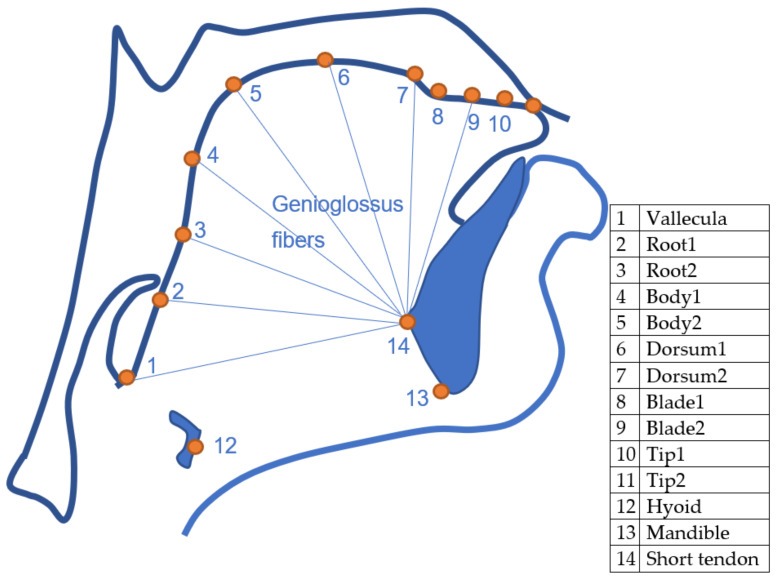
\includegraphics[keepaspectratio]{img/sensors-22-01133-g002.jpg}}

}

\caption{\label{fig-knots}Schematic representation of the knots tracked
by DeepLabCut.}

\end{figure}%

\subsection{GAM}\label{gam}

Generalised additive models (GAMs) are an extension of generalised
models that allow flexible modelling of non-linear effects (Hastie and
Tibshirani 1986; Wood 2006). GAMs are built upon smoothing splines
functions, the components of which are multiplied by estimated
coefficients to reconstruct an arbitrary time-changing curve. For a
thorough introduction to GAMs we refer the reader to (Sóskuthy 2021b,
2021a; Pedersen et al. 2019; Wieling 2018).

The data tracked by DeepLabCut consists of the position on the
horizontal (\emph{x}) and vertical (\emph{y}) axes of the fourteen
knots. In this tutorial, we will focus on modelling the tongue contour
based on the 11 knots from the vallecula to the tongue tip.
Figure~\ref{fig-tongue} illustrates the reconstructed tongue contour on
the basis of the 11 knots: the shown tongue is from the offset of a
vowel {[}o{]} followed by {[}t{]}, uttered by a Polish speaker (see
below for details on the data).

\phantomsection\label{cell-fig-tongue}
\begin{Shaded}
\begin{Highlighting}[]
\NormalTok{dlc\_voff\_f }\OtherTok{\textless{}{-}} \FunctionTok{readRDS}\NormalTok{(}\StringTok{"data/coretta2018/dlc\_voff\_f.rds"}\NormalTok{)}

\NormalTok{dlc\_voff\_f }\SpecialCharTok{|\textgreater{}} 
  \FunctionTok{filter}\NormalTok{(speaker }\SpecialCharTok{==} \StringTok{"pl04"}\NormalTok{, frame\_id }\SpecialCharTok{==} \DecValTok{432}\NormalTok{) }\SpecialCharTok{|\textgreater{}} 
  \FunctionTok{ggplot}\NormalTok{(}\FunctionTok{aes}\NormalTok{(X, Y, }\AttributeTok{group =}\NormalTok{ frame\_id)) }\SpecialCharTok{+}
  \FunctionTok{geom\_point}\NormalTok{() }\SpecialCharTok{+}
  \FunctionTok{geom\_path}\NormalTok{() }\SpecialCharTok{+}
  \FunctionTok{coord\_fixed}\NormalTok{() }\SpecialCharTok{+}
  \FunctionTok{labs}\NormalTok{(}\AttributeTok{x =} \StringTok{"X (mm)"}\NormalTok{, }\AttributeTok{y =} \StringTok{"Y (mm)"}\NormalTok{)}
\end{Highlighting}
\end{Shaded}

\begin{figure}[H]

\centering{

\pandocbounded{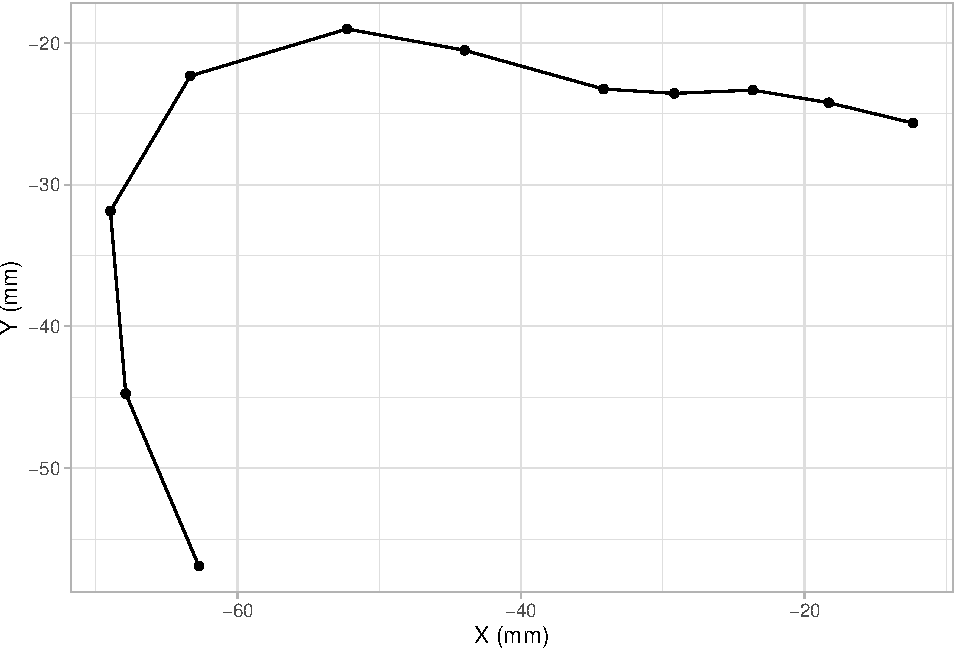
\includegraphics[keepaspectratio]{index_files/figure-pdf/fig-tongue-1.pdf}}

}

\caption{\label{fig-tongue}The eleven knots on the tongue contour taken
from the offset of {[}o{]} followed by {[}t{]} (Polish speaker PL04,
tongue tip to the right).}

\end{figure}%

\textsubscript{Source:
\href{https://stefanocoretta.github.io/mv_uti/index.qmd.html}{Article
Notebook}}

The same data is shown in Figure~\ref{fig-tongue-xy}, but in a different
format. Instead of a Cartesian coordinate system of X and Y values, the
plot has knot number on the \emph{x}-axis and X/Y coordinates on the
\emph{y}-axis. The X/Y coordinates thus form ``trajectories'' along the
knots. These trajectories are the ones that can be modelled using GAMs
and Functional Principal Component Analysis (FPCA). In this section, we
will illustrate GAMs applied to the X/Y trajectories along the knots and
how we can reconstruct the tongue contour from the modelled
trajectories. We will use data from two case studies of coarticulation:
vowel consonant (VC) coarticulation based on C place in Italian and
Polish, and consonantal articulation of plain vs emphatic consonants in
Lebanese Arabic.

\phantomsection\label{cell-fig-tongue-xy}
\begin{Shaded}
\begin{Highlighting}[]
\NormalTok{dlc\_voff\_f }\SpecialCharTok{|\textgreater{}} 
  \FunctionTok{filter}\NormalTok{(speaker }\SpecialCharTok{==} \StringTok{"pl04"}\NormalTok{, frame\_id }\SpecialCharTok{==} \DecValTok{432}\NormalTok{) }\SpecialCharTok{|\textgreater{}} 
\NormalTok{  dplyr}\SpecialCharTok{::}\FunctionTok{select}\NormalTok{(knot, X, Y) }\SpecialCharTok{|\textgreater{}} 
  \FunctionTok{pivot\_longer}\NormalTok{(}\FunctionTok{c}\NormalTok{(X,Y)) }\SpecialCharTok{|\textgreater{}} 
  \FunctionTok{ggplot}\NormalTok{(}\FunctionTok{aes}\NormalTok{(knot }\SpecialCharTok{+} \DecValTok{1}\NormalTok{, value)) }\SpecialCharTok{+}
  \FunctionTok{geom\_point}\NormalTok{() }\SpecialCharTok{+}
  \FunctionTok{geom\_path}\NormalTok{() }\SpecialCharTok{+}
  \FunctionTok{facet\_grid}\NormalTok{(}\AttributeTok{rows =} \FunctionTok{vars}\NormalTok{(name)) }\SpecialCharTok{+}
  \FunctionTok{scale\_x\_continuous}\NormalTok{(}\AttributeTok{breaks =} \DecValTok{1}\SpecialCharTok{:}\DecValTok{11}\NormalTok{) }\SpecialCharTok{+}
  \FunctionTok{labs}\NormalTok{(}\AttributeTok{x =} \StringTok{"Knot"}\NormalTok{, }\AttributeTok{y =} \StringTok{"Position (mm)"}\NormalTok{)}
\end{Highlighting}
\end{Shaded}

\begin{figure}[H]

\centering{

\pandocbounded{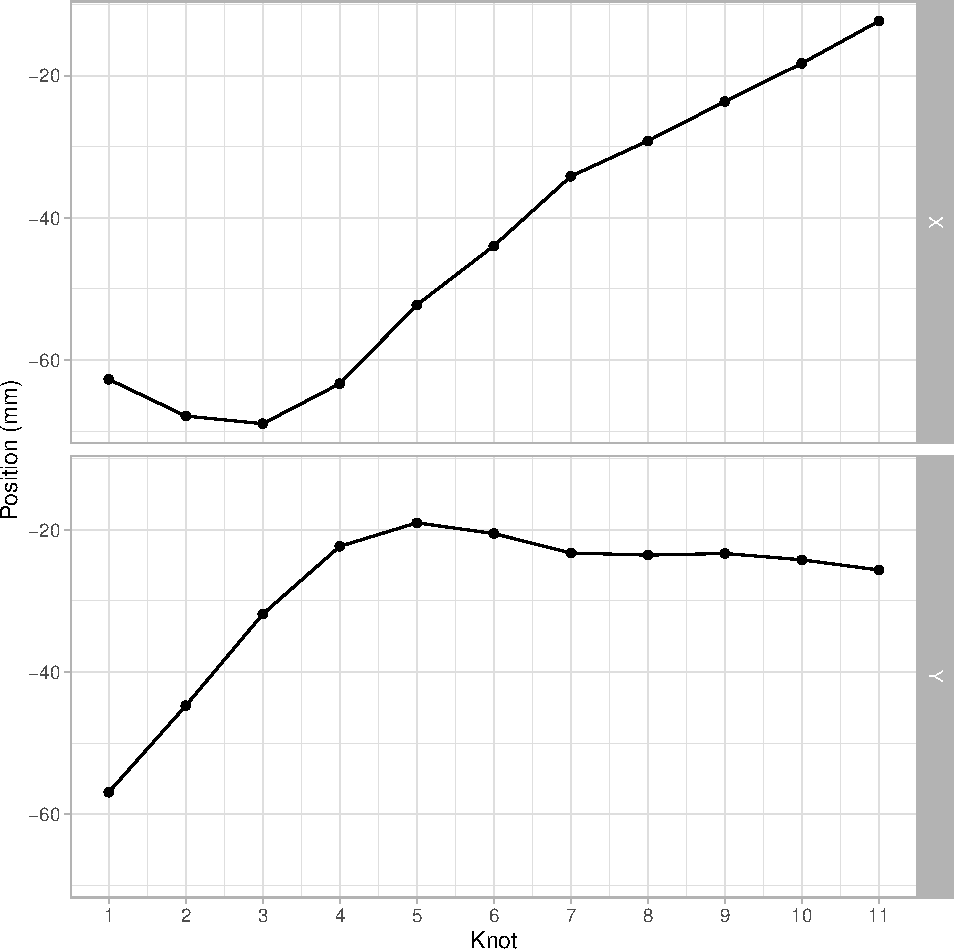
\includegraphics[keepaspectratio]{index_files/figure-pdf/fig-tongue-xy-1.pdf}}

}

\caption{\label{fig-tongue-xy}The horizontal and vertical positions of
the elevel knots (same data as Figure~\ref{fig-tongue}).}

\end{figure}%

\textsubscript{Source:
\href{https://stefanocoretta.github.io/mv_uti/index.qmd.html}{Article
Notebook}}

\subsubsection{VC coarticulation}\label{vc-coarticulation}

The data of the first case study, Coretta (2018), comes from Coretta
(2020b) and have been discussed in Coretta (2020a) (the analysis
concerned the position of the tongue root during the duration of vowels
followed by voiceless or voiced stops; in this paper we focus on tongue
contours at the vowel offset). The materials are /pVCV/ words embedded
in a frame sentence (\emph{Dico X lentamente} `I say X slowly' in
Italian and \emph{Mówię X teraz} `I say X now' in Polish). In the /pVCV/
words, C was /t, d, k, ɡ/ and V was /a, o, u/ (in each word, the two
vowels where identical, so for example \emph{pata, poto, putu}). The
data analysed here is from 9 speakers of Italian and 6 speakers of
Polish (other speakers were not included due to the difficulty in
processing their data with DeepLabCut).

{[}XXX Processing of data with DLC and filtering. Link to notebook{]}.

The following code chunk reads the filtered data. A sample of the data
is shown in Table~\ref{tbl-dlc-voff}. Figure~\ref{fig-voff} shows the
tongue contours for each individual speaker. It is possible to notice
clusters of different contours, related to each of the vowels /a, o, u/.
Figure~\ref{fig-pl04} zooms in on PL04 (Polish): the contours of each
vowel are coloured separately, and two panels separate tongue contours
taken at the offset of vowels followed by coronal (/t, d/) and velar
stops (/k, ɡ/). Crucially, the variation in tongue shape at vowel offset
(or closure onset) across vowels contexts is higher in the coronal than
in the velar contexts. This is not surprising, giving the greater
involvement of the tongue body and dorsum (the relevant articulators of
vowel production) in velar than in coronal stops.

\begin{Shaded}
\begin{Highlighting}[]
\NormalTok{dlc\_voff\_f }\OtherTok{\textless{}{-}} \FunctionTok{readRDS}\NormalTok{(}\StringTok{"data/coretta2018/dlc\_voff\_f.rds"}\NormalTok{)}
\end{Highlighting}
\end{Shaded}

\textsubscript{Source:
\href{https://stefanocoretta.github.io/mv_uti/index.qmd.html}{Article
Notebook}}

\begin{Shaded}
\begin{Highlighting}[]
\FunctionTok{head}\NormalTok{(dlc\_voff\_f }\SpecialCharTok{|\textgreater{}} \FunctionTok{select}\NormalTok{(speaker, word, X, Y, knot, knot\_label)) }\SpecialCharTok{|\textgreater{}} \FunctionTok{kable}\NormalTok{()}
\end{Highlighting}
\end{Shaded}

\begin{longtable}[]{@{}llrrrl@{}}

\caption{\label{tbl-dlc-voff}A sample of the VC coarticulation data from
Coretta (2018).}

\tabularnewline

\toprule\noalign{}
speaker & word & X & Y & knot & knot\_label \\
\midrule\noalign{}
\endhead
\bottomrule\noalign{}
\endlastfoot
it01 & pugu & -55.2105 & -44.1224 & 0 & Vallecula \\
it01 & pugu & -60.6994 & -31.3486 & 1 & Root\_1 \\
it01 & pugu & -65.1434 & -17.7311 & 2 & Root\_2 \\
it01 & pugu & -63.6757 & -4.2022 & 3 & Body\_1 \\
it01 & pugu & -57.2505 & 7.8483 & 4 & Body\_2 \\
it01 & pugu & -44.9086 & 13.3162 & 5 & Dorsum\_1 \\

\end{longtable}

\textsubscript{Source:
\href{https://stefanocoretta.github.io/mv_uti/index.qmd.html}{Article
Notebook}}

\phantomsection\label{cell-fig-voff}
\begin{Shaded}
\begin{Highlighting}[]
\NormalTok{dlc\_voff\_f }\SpecialCharTok{|\textgreater{}} 
  \FunctionTok{ggplot}\NormalTok{(}\FunctionTok{aes}\NormalTok{(X\_z, Y\_z, }\AttributeTok{group =}\NormalTok{ frame\_id)) }\SpecialCharTok{+}
  \FunctionTok{geom\_path}\NormalTok{(}\AttributeTok{alpha =} \FloatTok{0.25}\NormalTok{) }\SpecialCharTok{+}
  \FunctionTok{coord\_fixed}\NormalTok{() }\SpecialCharTok{+}
  \FunctionTok{facet\_wrap}\NormalTok{(}\FunctionTok{vars}\NormalTok{(speaker), }\AttributeTok{ncol =} \DecValTok{5}\NormalTok{)}
\end{Highlighting}
\end{Shaded}

\begin{figure}[H]

\centering{

\pandocbounded{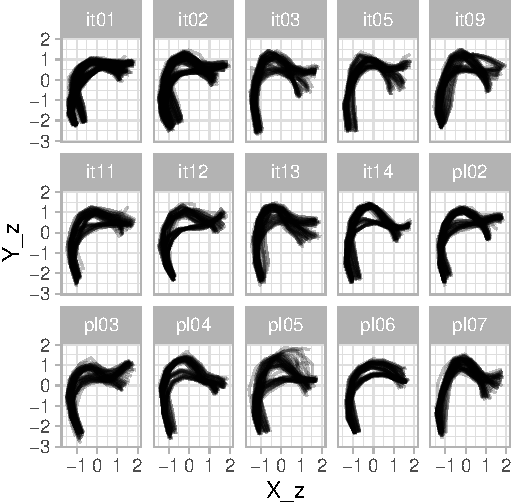
\includegraphics[keepaspectratio]{index_files/figure-pdf/fig-voff-1.pdf}}

}

\caption{\label{fig-voff}Tongue contours of 9 Italian speakers and6
Polish speakers, taken from the offset of the first vowel in /pCVCV/
target words.}

\end{figure}%

\textsubscript{Source:
\href{https://stefanocoretta.github.io/mv_uti/index.qmd.html}{Article
Notebook}}

\phantomsection\label{cell-fig-pl04}
\begin{Shaded}
\begin{Highlighting}[]
\NormalTok{dlc\_voff\_f }\SpecialCharTok{|\textgreater{}} 
  \FunctionTok{filter}\NormalTok{(speaker }\SpecialCharTok{==} \StringTok{"pl04"}\NormalTok{) }\SpecialCharTok{|\textgreater{}} 
  \FunctionTok{ggplot}\NormalTok{(}\FunctionTok{aes}\NormalTok{(X\_z, Y\_z, }\AttributeTok{group =}\NormalTok{ frame\_id, }\AttributeTok{colour =}\NormalTok{ vowel)) }\SpecialCharTok{+}
  \FunctionTok{geom\_path}\NormalTok{(}\AttributeTok{alpha =} \FloatTok{0.5}\NormalTok{) }\SpecialCharTok{+}
  \FunctionTok{coord\_fixed}\NormalTok{() }\SpecialCharTok{+}
  \FunctionTok{facet\_grid}\NormalTok{(}\AttributeTok{cols =} \FunctionTok{vars}\NormalTok{(c2\_place)) }\SpecialCharTok{+}
  \FunctionTok{labs}\NormalTok{(}\AttributeTok{x =} \StringTok{"X (z{-}scores)"}\NormalTok{, }\StringTok{"Y (z{-}scores)"}\NormalTok{)}
\end{Highlighting}
\end{Shaded}

\begin{figure}[H]

\centering{

\pandocbounded{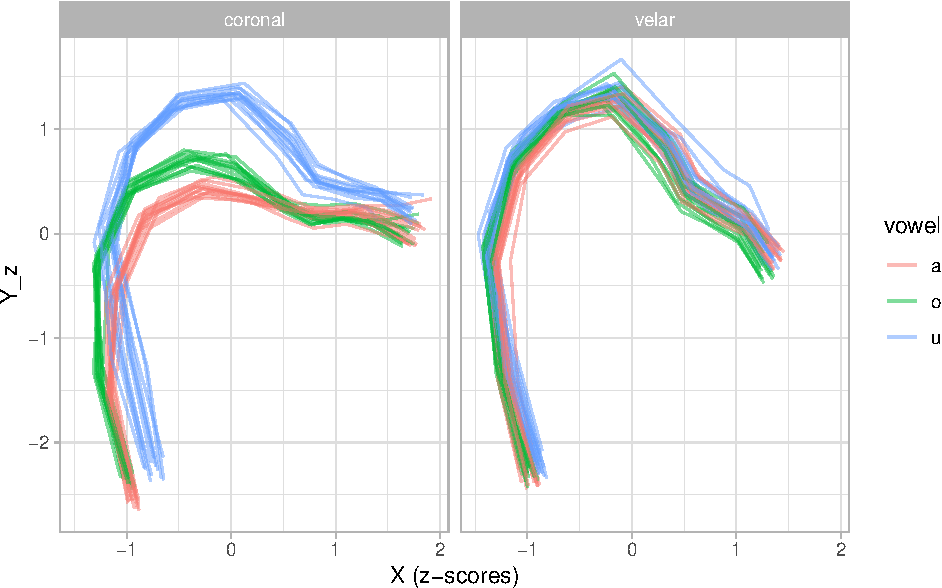
\includegraphics[keepaspectratio]{index_files/figure-pdf/fig-pl04-1.pdf}}

}

\caption{\label{fig-pl04}Tongue contours of PL04 (Polish) taken from the
offset of vowels followed by coronal or velar stops. Tip is on the
right.}

\end{figure}%

\textsubscript{Source:
\href{https://stefanocoretta.github.io/mv_uti/index.qmd.html}{Article
Notebook}}

\begin{Shaded}
\begin{Highlighting}[]
\FunctionTok{library}\NormalTok{(mgcv)}
\end{Highlighting}
\end{Shaded}

\begin{verbatim}
Loading required package: nlme
\end{verbatim}

\begin{verbatim}

Attaching package: 'nlme'
\end{verbatim}

\begin{verbatim}
The following object is masked from 'package:dplyr':

    collapse
\end{verbatim}

\begin{verbatim}
This is mgcv 1.9-1. For overview type 'help("mgcv-package")'.
\end{verbatim}

\begin{Shaded}
\begin{Highlighting}[]
\NormalTok{fi }\OtherTok{\textless{}{-}} \StringTok{"data/cache/voff\_gam.rds"}

\ControlFlowTok{if}\NormalTok{ (}\FunctionTok{file.exists}\NormalTok{(fi)) \{}
\NormalTok{  voff\_gam }\OtherTok{\textless{}{-}} \FunctionTok{readRDS}\NormalTok{(fi)}
\NormalTok{\} }\ControlFlowTok{else}\NormalTok{ \{}
\NormalTok{  voff\_gam }\OtherTok{\textless{}{-}} \FunctionTok{gam}\NormalTok{(}
    \FunctionTok{list}\NormalTok{(}
\NormalTok{      X\_z }\SpecialCharTok{\textasciitilde{}}\NormalTok{ vow\_place\_lang }\SpecialCharTok{+}
        \FunctionTok{s}\NormalTok{(knot, }\AttributeTok{by =}\NormalTok{ vow\_place\_lang, }\AttributeTok{k =} \DecValTok{5}\NormalTok{) }\SpecialCharTok{+}
        \FunctionTok{s}\NormalTok{(knot, speaker, }\AttributeTok{by =}\NormalTok{ vow\_place, }\AttributeTok{bs =} \StringTok{"fs"}\NormalTok{, }\AttributeTok{m =} \DecValTok{1}\NormalTok{),}
\NormalTok{      Y\_z }\SpecialCharTok{\textasciitilde{}}\NormalTok{ vow\_place\_lang }\SpecialCharTok{+}
        \FunctionTok{s}\NormalTok{(knot, }\AttributeTok{by =}\NormalTok{ vow\_place\_lang, }\AttributeTok{k =} \DecValTok{5}\NormalTok{) }\SpecialCharTok{+}
        \FunctionTok{s}\NormalTok{(knot, speaker, }\AttributeTok{by =}\NormalTok{ vow\_place, }\AttributeTok{bs =} \StringTok{"fs"}\NormalTok{, }\AttributeTok{m =} \DecValTok{1}\NormalTok{)}
\NormalTok{    ),}
    \AttributeTok{data =}\NormalTok{ dlc\_voff\_f,}
    \AttributeTok{family =} \FunctionTok{mvn}\NormalTok{(}\AttributeTok{d =} \DecValTok{2}\NormalTok{)}
\NormalTok{  )}
  
  \FunctionTok{saveRDS}\NormalTok{(voff\_gam, fi)}
\NormalTok{\}}
\end{Highlighting}
\end{Shaded}

\textsubscript{Source:
\href{https://stefanocoretta.github.io/mv_uti/index.qmd.html}{Article
Notebook}}

\begin{Shaded}
\begin{Highlighting}[]
\NormalTok{frame\_voff }\OtherTok{\textless{}{-}} \FunctionTok{expand\_grid}\NormalTok{(}
  \AttributeTok{speaker =} \FunctionTok{unique}\NormalTok{(dlc\_voff\_f}\SpecialCharTok{$}\NormalTok{speaker),}
  \AttributeTok{vow\_place\_lang =} \FunctionTok{unique}\NormalTok{(dlc\_voff\_f}\SpecialCharTok{$}\NormalTok{vow\_place\_lang),}
  \AttributeTok{knot =} \FunctionTok{seq}\NormalTok{(}\DecValTok{0}\NormalTok{, }\DecValTok{10}\NormalTok{, }\AttributeTok{by =} \FloatTok{0.1}\NormalTok{)}
\NormalTok{) }\SpecialCharTok{|\textgreater{}} 
  \FunctionTok{mutate}\NormalTok{(}
    \AttributeTok{vow\_place =} \FunctionTok{str\_remove}\NormalTok{(vow\_place\_lang, }\StringTok{"}\SpecialCharTok{\textbackslash{}\textbackslash{}}\StringTok{.Italian"}\NormalTok{),}
    \AttributeTok{vow\_place =} \FunctionTok{str\_remove}\NormalTok{(vow\_place, }\StringTok{"}\SpecialCharTok{\textbackslash{}\textbackslash{}}\StringTok{.Polish"}\NormalTok{),}
\NormalTok{  )}

\NormalTok{excl }\OtherTok{\textless{}{-}} \FunctionTok{c}\NormalTok{(}
  \StringTok{"s(knot,speaker):vow\_placea.coronal"}\NormalTok{,}
  \StringTok{"s(knot,speaker):vow\_placeo.coronal"}\NormalTok{,}
  \StringTok{"s(knot,speaker):vow\_placeu.coronal"}\NormalTok{,}
  \StringTok{"s(knot,speaker):vow\_placea.velar"}\NormalTok{,}
  \StringTok{"s(knot,speaker):vow\_placeo.velar"}\NormalTok{,}
  \StringTok{"s(knot,speaker):vow\_placeu.velar"}\NormalTok{,}
  \StringTok{"s.1(knot,speaker):vow\_placea.coronal"}\NormalTok{,}
  \StringTok{"s.1(knot,speaker):vow\_placeo.coronal"}\NormalTok{,}
  \StringTok{"s.1(knot,speaker):vow\_placeu.coronal"}\NormalTok{,}
  \StringTok{"s.1(knot,speaker):vow\_placea.velar"}\NormalTok{,}
  \StringTok{"s.1(knot,speaker):vow\_placeo.velar"}\NormalTok{,}
  \StringTok{"s.1(knot,speaker):vow\_placeu.velar"}
\NormalTok{)}

\NormalTok{voff\_gam\_p }\OtherTok{\textless{}{-}} \FunctionTok{predict}\NormalTok{(voff\_gam, frame\_voff, }\AttributeTok{se.fit =} \ConstantTok{TRUE}\NormalTok{, }\AttributeTok{exclude =}\NormalTok{ excl) }\SpecialCharTok{|\textgreater{}}
  \FunctionTok{as.data.frame}\NormalTok{() }\SpecialCharTok{|\textgreater{}}
  \FunctionTok{as\_tibble}\NormalTok{()}
\FunctionTok{colnames}\NormalTok{(voff\_gam\_p) }\OtherTok{\textless{}{-}} \FunctionTok{c}\NormalTok{(}\StringTok{"X"}\NormalTok{, }\StringTok{"Y"}\NormalTok{, }\StringTok{"X\_se"}\NormalTok{, }\StringTok{"Y\_se"}\NormalTok{)}

\NormalTok{voff\_gam\_p }\OtherTok{\textless{}{-}} \FunctionTok{bind\_cols}\NormalTok{(frame\_voff, voff\_gam\_p) }\SpecialCharTok{|\textgreater{}} 
  \CommentTok{\# pick any speaker, random effects have been removed}
  \FunctionTok{filter}\NormalTok{(speaker }\SpecialCharTok{==} \StringTok{"it01"}\NormalTok{) }\SpecialCharTok{|\textgreater{}} 
  \FunctionTok{mutate}\NormalTok{(}
    \AttributeTok{X\_lo =}\NormalTok{ X }\SpecialCharTok{{-}}\NormalTok{ (}\FloatTok{1.96} \SpecialCharTok{*}\NormalTok{ X\_se),}
    \AttributeTok{X\_hi =}\NormalTok{ X }\SpecialCharTok{+}\NormalTok{ (}\FloatTok{1.96} \SpecialCharTok{*}\NormalTok{ X\_se),}
    \AttributeTok{Y\_lo =}\NormalTok{ Y }\SpecialCharTok{{-}}\NormalTok{ (}\FloatTok{1.96} \SpecialCharTok{*}\NormalTok{ Y\_se),}
    \AttributeTok{Y\_hi =}\NormalTok{ Y }\SpecialCharTok{+}\NormalTok{ (}\FloatTok{1.96} \SpecialCharTok{*}\NormalTok{ Y\_se)}
\NormalTok{  ) }\SpecialCharTok{|\textgreater{}} 
  \FunctionTok{separate}\NormalTok{(vow\_place\_lang, }\FunctionTok{c}\NormalTok{(}\StringTok{"vowel"}\NormalTok{, }\StringTok{"place"}\NormalTok{, }\StringTok{"language"}\NormalTok{))}
\end{Highlighting}
\end{Shaded}

\textsubscript{Source:
\href{https://stefanocoretta.github.io/mv_uti/index.qmd.html}{Article
Notebook}}

\phantomsection\label{cell-fig-voff-pred}
\begin{Shaded}
\begin{Highlighting}[]
\NormalTok{voff\_gam\_p }\SpecialCharTok{|\textgreater{}} 
  \FunctionTok{ggplot}\NormalTok{(}\FunctionTok{aes}\NormalTok{(X, Y, }\AttributeTok{colour =}\NormalTok{ vowel)) }\SpecialCharTok{+}
  \FunctionTok{geom\_point}\NormalTok{(}\AttributeTok{alpha =} \FloatTok{0.5}\NormalTok{) }\SpecialCharTok{+}
  \FunctionTok{facet\_grid}\NormalTok{(}\AttributeTok{cols =} \FunctionTok{vars}\NormalTok{(place), }\AttributeTok{rows =} \FunctionTok{vars}\NormalTok{(language)) }\SpecialCharTok{+}
  \FunctionTok{coord\_fixed}\NormalTok{() }\SpecialCharTok{+}
  \FunctionTok{labs}\NormalTok{(}
    \AttributeTok{x =} \StringTok{"X (z{-}scores)"}\NormalTok{,}
    \AttributeTok{y =} \StringTok{"Y (z{-}scores)"}
\NormalTok{  )}
\end{Highlighting}
\end{Shaded}

\begin{figure}[H]

\centering{

\pandocbounded{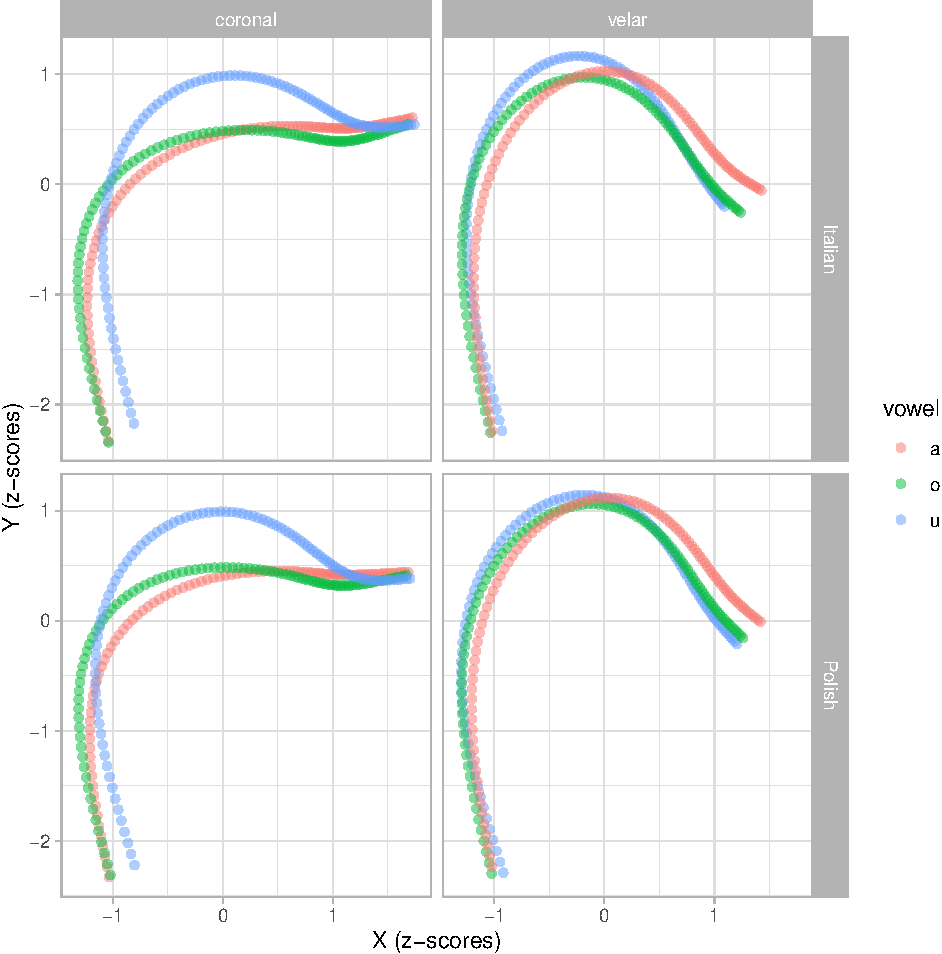
\includegraphics[keepaspectratio]{index_files/figure-pdf/fig-voff-pred-1.pdf}}

}

\caption{\label{fig-voff-pred}Predicted tongue contours based on a
multivariate GAM. Uncertainty not shown.}

\end{figure}%

\textsubscript{Source:
\href{https://stefanocoretta.github.io/mv_uti/index.qmd.html}{Article
Notebook}}

\phantomsection\label{cell-fig-voff-ci}
\begin{Shaded}
\begin{Highlighting}[]
\NormalTok{voff\_gam\_p }\SpecialCharTok{|\textgreater{}} 
  \FunctionTok{group\_by}\NormalTok{(place, vowel, language) }\SpecialCharTok{|\textgreater{}} 
  \FunctionTok{mutate}\NormalTok{(}
    \AttributeTok{Y\_lo =} \FunctionTok{ifelse}\NormalTok{(Y\_lo }\SpecialCharTok{\textgreater{}} \FunctionTok{min}\NormalTok{(Y), Y\_lo, }\ConstantTok{NA}\NormalTok{),}
    \AttributeTok{X\_hi =} \FunctionTok{ifelse}\NormalTok{(X\_hi }\SpecialCharTok{\textless{}} \FunctionTok{max}\NormalTok{(X), X\_hi, }\ConstantTok{NA}\NormalTok{),}
\NormalTok{  ) }\SpecialCharTok{|\textgreater{}} 
  \FunctionTok{ggplot}\NormalTok{(}\FunctionTok{aes}\NormalTok{(X, Y, }\AttributeTok{colour =}\NormalTok{ vowel)) }\SpecialCharTok{+}
  \FunctionTok{geom\_errorbarh}\NormalTok{(}\FunctionTok{aes}\NormalTok{(}\AttributeTok{xmin =}\NormalTok{ X\_lo, }\AttributeTok{xmax =}\NormalTok{ X\_hi), }\AttributeTok{alpha =} \FloatTok{0.5}\NormalTok{) }\SpecialCharTok{+}
  \FunctionTok{geom\_errorbar}\NormalTok{(}\FunctionTok{aes}\NormalTok{(}\AttributeTok{ymin =}\NormalTok{ Y\_lo, }\AttributeTok{ymax =}\NormalTok{ Y\_hi), }\AttributeTok{alpha =} \FloatTok{0.5}\NormalTok{) }\SpecialCharTok{+}
  \FunctionTok{geom\_point}\NormalTok{(}\AttributeTok{size =} \DecValTok{1}\NormalTok{, }\AttributeTok{alpha =} \FloatTok{0.75}\NormalTok{) }\SpecialCharTok{+}
  \FunctionTok{scale\_color\_brewer}\NormalTok{(}\AttributeTok{type =} \StringTok{"qual"}\NormalTok{, }\AttributeTok{palette =} \StringTok{"Dark2"}\NormalTok{) }\SpecialCharTok{+}
  \FunctionTok{coord\_fixed}\NormalTok{() }\SpecialCharTok{+}
  \FunctionTok{facet\_grid}\NormalTok{(}\AttributeTok{cols =} \FunctionTok{vars}\NormalTok{(place), }\AttributeTok{rows =} \FunctionTok{vars}\NormalTok{(language)) }\SpecialCharTok{+}
  \FunctionTok{theme\_light}\NormalTok{() }\SpecialCharTok{+}
  \FunctionTok{theme}\NormalTok{(}\AttributeTok{legend.position =} \StringTok{"bottom"}\NormalTok{)}
\end{Highlighting}
\end{Shaded}

\begin{verbatim}
Warning: Removed 57 rows containing missing values or values outside the scale range
(`geom_errorbarh()`).
\end{verbatim}

\begin{figure}[H]

\centering{

\pandocbounded{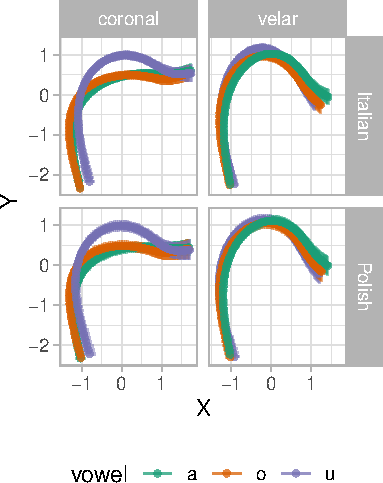
\includegraphics[keepaspectratio]{index_files/figure-pdf/fig-voff-ci-1.pdf}}

}

\caption{\label{fig-voff-ci}Predicted tongue contours based on a
multivariate GAM, with 95\% Confidence Intervals.}

\end{figure}%

\textsubscript{Source:
\href{https://stefanocoretta.github.io/mv_uti/index.qmd.html}{Article
Notebook}}

\begin{Shaded}
\begin{Highlighting}[]
\NormalTok{frame\_voff }\OtherTok{\textless{}{-}} \FunctionTok{expand\_grid}\NormalTok{(}
  \AttributeTok{speaker =} \FunctionTok{unique}\NormalTok{(dlc\_voff\_f}\SpecialCharTok{$}\NormalTok{speaker),}
  \AttributeTok{vow\_place\_lang =} \FunctionTok{unique}\NormalTok{(dlc\_voff\_f}\SpecialCharTok{$}\NormalTok{vow\_place\_lang),}
  \AttributeTok{knot =} \FunctionTok{seq}\NormalTok{(}\DecValTok{0}\NormalTok{, }\DecValTok{10}\NormalTok{)}
\NormalTok{) }\SpecialCharTok{|\textgreater{}} 
  \FunctionTok{mutate}\NormalTok{(}
    \AttributeTok{vow\_place =} \FunctionTok{str\_remove}\NormalTok{(vow\_place\_lang, }\StringTok{"}\SpecialCharTok{\textbackslash{}\textbackslash{}}\StringTok{.Italian"}\NormalTok{),}
    \AttributeTok{vow\_place =} \FunctionTok{str\_remove}\NormalTok{(vow\_place, }\StringTok{"}\SpecialCharTok{\textbackslash{}\textbackslash{}}\StringTok{.Polish"}\NormalTok{),}
\NormalTok{  )}

\NormalTok{pred\_grid\_a }\OtherTok{\textless{}{-}} \FunctionTok{filter}\NormalTok{(}
\NormalTok{  frame\_voff, vow\_place\_lang }\SpecialCharTok{==} \StringTok{"a.coronal.Italian"}\NormalTok{,}
\NormalTok{  speaker }\SpecialCharTok{==} \StringTok{"it01"}
\NormalTok{)}
\NormalTok{pred\_grid\_b }\OtherTok{\textless{}{-}} \FunctionTok{filter}\NormalTok{(}
\NormalTok{  frame\_voff, vow\_place\_lang }\SpecialCharTok{==} \StringTok{"u.coronal.Italian"}\NormalTok{,}
\NormalTok{  speaker }\SpecialCharTok{==} \StringTok{"it01"}
\NormalTok{)}

\NormalTok{pred\_a }\OtherTok{\textless{}{-}} \FunctionTok{predict.gam}\NormalTok{(voff\_gam, pred\_grid\_a, }\AttributeTok{type =} \StringTok{"lpmatrix"}\NormalTok{) }\SpecialCharTok{|\textgreater{}} 
  \FunctionTok{as\_tibble}\NormalTok{() }\SpecialCharTok{|\textgreater{}} 
  \FunctionTok{mutate}\NormalTok{(}
    \FunctionTok{across}\NormalTok{(}\FunctionTok{starts\_with}\NormalTok{(}\StringTok{"s(knot,speaker)"}\NormalTok{), }\SpecialCharTok{\textasciitilde{}}\DecValTok{0}\NormalTok{)}
\NormalTok{  ) }\SpecialCharTok{|\textgreater{}} 
  \FunctionTok{as.matrix}\NormalTok{()}
\NormalTok{pred\_a[,}\DecValTok{1}\SpecialCharTok{:}\DecValTok{870}\NormalTok{] }\OtherTok{\textless{}{-}} \DecValTok{0}

\NormalTok{pred\_b }\OtherTok{\textless{}{-}} \FunctionTok{predict.gam}\NormalTok{(voff\_gam, pred\_grid\_b, }\AttributeTok{type =} \StringTok{"lpmatrix"}\NormalTok{) }\SpecialCharTok{|\textgreater{}} 
  \FunctionTok{as\_tibble}\NormalTok{() }\SpecialCharTok{|\textgreater{}} 
  \FunctionTok{mutate}\NormalTok{(}
    \FunctionTok{across}\NormalTok{(}\FunctionTok{starts\_with}\NormalTok{(}\StringTok{"s(knot,speaker)"}\NormalTok{), }\SpecialCharTok{\textasciitilde{}}\DecValTok{0}\NormalTok{)}
\NormalTok{  ) }\SpecialCharTok{|\textgreater{}} 
  \FunctionTok{as.matrix}\NormalTok{()}
\NormalTok{pred\_b[,}\DecValTok{1}\SpecialCharTok{:}\DecValTok{870}\NormalTok{] }\OtherTok{\textless{}{-}} \DecValTok{0}

\NormalTok{pred\_diff }\OtherTok{\textless{}{-}}\NormalTok{ pred\_a }\SpecialCharTok{{-}}\NormalTok{ pred\_b}
\NormalTok{diff }\OtherTok{\textless{}{-}} \FunctionTok{as.vector}\NormalTok{(pred\_diff }\SpecialCharTok{\%*\%}\NormalTok{ stats}\SpecialCharTok{::}\FunctionTok{coef}\NormalTok{(voff\_gam))}

\NormalTok{se }\OtherTok{\textless{}{-}} \FunctionTok{sqrt}\NormalTok{(}\FunctionTok{rowSums}\NormalTok{((pred\_diff }\SpecialCharTok{\%*\%}\NormalTok{ stats}\SpecialCharTok{::}\FunctionTok{vcov}\NormalTok{(voff\_gam)) }\SpecialCharTok{*}\NormalTok{ pred\_diff))}

\NormalTok{diff\_out }\OtherTok{\textless{}{-}}\NormalTok{ pred\_grid\_a}
\NormalTok{diff\_out}\SpecialCharTok{$}\NormalTok{diff }\OtherTok{\textless{}{-}}\NormalTok{ diff}
\NormalTok{diff\_out}\SpecialCharTok{$}\NormalTok{se }\OtherTok{\textless{}{-}}\NormalTok{ se}
\NormalTok{diff\_out}\SpecialCharTok{$}\NormalTok{lower\_ci }\OtherTok{\textless{}{-}}\NormalTok{ diff }\SpecialCharTok{{-}}\NormalTok{ se }\SpecialCharTok{*} \FloatTok{1.96}
\NormalTok{diff\_out}\SpecialCharTok{$}\NormalTok{upper\_ci }\OtherTok{\textless{}{-}}\NormalTok{ diff }\SpecialCharTok{+}\NormalTok{ se }\SpecialCharTok{*} \FloatTok{1.96}
\end{Highlighting}
\end{Shaded}

\textsubscript{Source:
\href{https://stefanocoretta.github.io/mv_uti/index.qmd.html}{Article
Notebook}}

\begin{Shaded}
\begin{Highlighting}[]
\NormalTok{diff\_out }\SpecialCharTok{|\textgreater{}} 
  \FunctionTok{ggplot}\NormalTok{(}\FunctionTok{aes}\NormalTok{(knot, diff)) }\SpecialCharTok{+}
  \FunctionTok{geom\_hline}\NormalTok{(}\AttributeTok{yintercept =} \DecValTok{0}\NormalTok{) }\SpecialCharTok{+}
  \FunctionTok{geom\_ribbon}\NormalTok{(}\FunctionTok{aes}\NormalTok{(}\AttributeTok{ymin =}\NormalTok{ lower\_ci, }\AttributeTok{ymax =}\NormalTok{ upper\_ci), }\AttributeTok{alpha =} \FloatTok{0.5}\NormalTok{) }\SpecialCharTok{+}
  \FunctionTok{geom\_point}\NormalTok{()}
\end{Highlighting}
\end{Shaded}

\pandocbounded{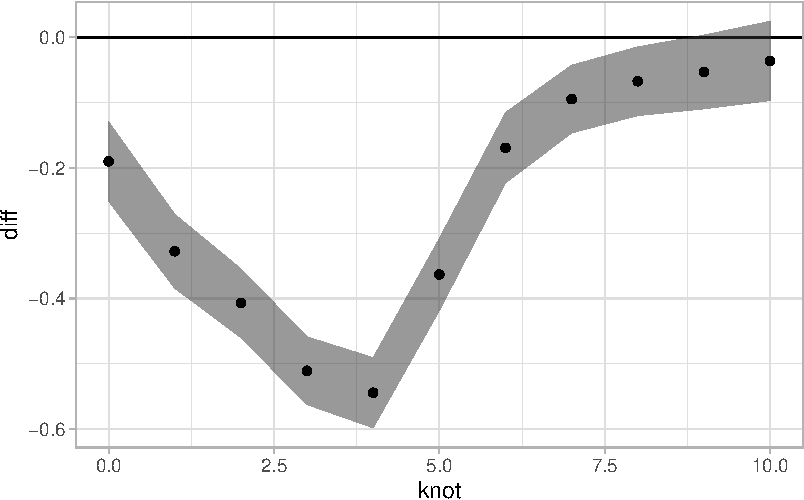
\includegraphics[keepaspectratio]{index_files/figure-pdf/unnamed-chunk-2-1.pdf}}

\textsubscript{Source:
\href{https://stefanocoretta.github.io/mv_uti/index.qmd.html}{Article
Notebook}}

\subsubsection{Emphaticness}\label{emphaticness}

\begin{Shaded}
\begin{Highlighting}[]
\NormalTok{dlc\_emph\_f }\OtherTok{\textless{}{-}} \FunctionTok{readRDS}\NormalTok{(}\StringTok{"data/sakr2025/dlc\_emph\_f.rds"}\NormalTok{)}
\end{Highlighting}
\end{Shaded}

\textsubscript{Source:
\href{https://stefanocoretta.github.io/mv_uti/index.qmd.html}{Article
Notebook}}

\begin{Shaded}
\begin{Highlighting}[]
\FunctionTok{library}\NormalTok{(mgcv)}

\NormalTok{fi }\OtherTok{\textless{}{-}} \StringTok{"data/cache/emph\_gam.rds"}

\ControlFlowTok{if}\NormalTok{ (}\FunctionTok{file.exists}\NormalTok{(fi)) \{}
\NormalTok{  emph\_gam }\OtherTok{\textless{}{-}} \FunctionTok{readRDS}\NormalTok{(fi)}
\NormalTok{\} }\ControlFlowTok{else}\NormalTok{ \{}
\NormalTok{  emph\_gam }\OtherTok{\textless{}{-}} \FunctionTok{gam}\NormalTok{(}
    \FunctionTok{list}\NormalTok{(}
\NormalTok{      X\_z }\SpecialCharTok{\textasciitilde{}}\NormalTok{ vow\_emph }\SpecialCharTok{+}
        \FunctionTok{s}\NormalTok{(knot, }\AttributeTok{by =}\NormalTok{ vow\_emph, }\AttributeTok{k =} \DecValTok{5}\NormalTok{) }\SpecialCharTok{+}
        \FunctionTok{s}\NormalTok{(knot, participant, }\AttributeTok{by =}\NormalTok{ vow\_emph, }\AttributeTok{bs =} \StringTok{"fs"}\NormalTok{, }\AttributeTok{m =} \DecValTok{1}\NormalTok{, }\AttributeTok{k =} \DecValTok{5}\NormalTok{),}
\NormalTok{      Y\_z }\SpecialCharTok{\textasciitilde{}}\NormalTok{ vow\_emph }\SpecialCharTok{+}
        \FunctionTok{s}\NormalTok{(knot, }\AttributeTok{by =}\NormalTok{ vow\_emph, }\AttributeTok{k =} \DecValTok{5}\NormalTok{) }\SpecialCharTok{+}
        \FunctionTok{s}\NormalTok{(knot, participant, }\AttributeTok{by =}\NormalTok{ vow\_emph, }\AttributeTok{bs =} \StringTok{"fs"}\NormalTok{, }\AttributeTok{m =} \DecValTok{1}\NormalTok{, }\AttributeTok{k =} \DecValTok{5}\NormalTok{)}
\NormalTok{    ),}
    \AttributeTok{data =}\NormalTok{ dlc\_emph\_f,}
    \AttributeTok{family =} \FunctionTok{mvn}\NormalTok{(}\AttributeTok{d =} \DecValTok{2}\NormalTok{)}
\NormalTok{  )}
  
  \FunctionTok{saveRDS}\NormalTok{(emph\_gam, fi)}
\NormalTok{\}}
\end{Highlighting}
\end{Shaded}

\textsubscript{Source:
\href{https://stefanocoretta.github.io/mv_uti/index.qmd.html}{Article
Notebook}}

\begin{Shaded}
\begin{Highlighting}[]
\NormalTok{frame\_emph }\OtherTok{\textless{}{-}} \FunctionTok{expand\_grid}\NormalTok{(}
  \AttributeTok{participant =} \FunctionTok{unique}\NormalTok{(dlc\_emph\_f}\SpecialCharTok{$}\NormalTok{participant),}
  \AttributeTok{vow\_emph =} \FunctionTok{unique}\NormalTok{(dlc\_emph\_f}\SpecialCharTok{$}\NormalTok{vow\_emph),}
  \AttributeTok{knot =} \FunctionTok{seq}\NormalTok{(}\DecValTok{0}\NormalTok{, }\DecValTok{10}\NormalTok{, }\AttributeTok{by =} \FloatTok{0.1}\NormalTok{)}
\NormalTok{)}

\NormalTok{excl }\OtherTok{\textless{}{-}} \FunctionTok{c}\NormalTok{(}
  \StringTok{"s(Knot,participant):vow\_emphA.Emphatic"}\NormalTok{,}
  \StringTok{"s(Knot,participant):vow\_emphE.Emphatic"}\NormalTok{,}
  \StringTok{"s(Knot,participant):vow\_emphI.Emphatic"}\NormalTok{,}
  \StringTok{"s(Knot,participant):vow\_emphO.Emphatic"}\NormalTok{,}
  \StringTok{"s(Knot,participant):vow\_emphU.Emphatic"}\NormalTok{,}
  \StringTok{"s.1(Knot,participant):vow\_emphA.Emphatic"}\NormalTok{,}
  \StringTok{"s.1(Knot,participant):vow\_emphE.Emphatic"}\NormalTok{,}
  \StringTok{"s.1(Knot,participant):vow\_emphI.Emphatic"}\NormalTok{,}
  \StringTok{"s.1(Knot,participant):vow\_emphO.Emphatic"}\NormalTok{,}
  \StringTok{"s.1(Knot,participant):vow\_emphU.Emphatic"}\NormalTok{,}
  \StringTok{"s(Knot,participant):vow\_emphA.Plain"}\NormalTok{,}
  \StringTok{"s(Knot,participant):vow\_emphE.Plain"}\NormalTok{,}
  \StringTok{"s(Knot,participant):vow\_emphI.Plain"}\NormalTok{,}
  \StringTok{"s(Knot,participant):vow\_emphO.Plain"}\NormalTok{,}
  \StringTok{"s(Knot,participant):vow\_emphU.Plain"}\NormalTok{,}
  \StringTok{"s.1(Knot,participant):vow\_emphA.Plain"}\NormalTok{,}
  \StringTok{"s.1(Knot,participant):vow\_emphE.Plain"}\NormalTok{,}
  \StringTok{"s.1(Knot,participant):vow\_emphI.Plain"}\NormalTok{,}
  \StringTok{"s.1(Knot,participant):vow\_emphO.Plain"}\NormalTok{,}
  \StringTok{"s.1(Knot,participant):vow\_emphU.Plain"}
\NormalTok{)}

\NormalTok{emph\_gam\_p }\OtherTok{\textless{}{-}} \FunctionTok{predict}\NormalTok{(emph\_gam, frame\_emph, }\AttributeTok{se.fit =} \ConstantTok{TRUE}\NormalTok{, }\AttributeTok{exclude =}\NormalTok{ excl) }\SpecialCharTok{|\textgreater{}}
  \FunctionTok{as.data.frame}\NormalTok{() }\SpecialCharTok{|\textgreater{}}
  \FunctionTok{as\_tibble}\NormalTok{()}
\FunctionTok{colnames}\NormalTok{(emph\_gam\_p) }\OtherTok{\textless{}{-}} \FunctionTok{c}\NormalTok{(}\StringTok{"X"}\NormalTok{, }\StringTok{"Y"}\NormalTok{, }\StringTok{"X\_se"}\NormalTok{, }\StringTok{"Y\_se"}\NormalTok{)}

\NormalTok{emph\_gam\_p }\OtherTok{\textless{}{-}} \FunctionTok{bind\_cols}\NormalTok{(frame\_emph, emph\_gam\_p) }\SpecialCharTok{|\textgreater{}} 
  \CommentTok{\# pick any speaker, random effects have been removed}
  \FunctionTok{filter}\NormalTok{(participant }\SpecialCharTok{==} \StringTok{"Sak"}\NormalTok{) }\SpecialCharTok{|\textgreater{}} 
  \FunctionTok{mutate}\NormalTok{(}
    \AttributeTok{X\_lo =}\NormalTok{ X }\SpecialCharTok{{-}}\NormalTok{ (}\FloatTok{1.96} \SpecialCharTok{*}\NormalTok{ X\_se),}
    \AttributeTok{X\_hi =}\NormalTok{ X }\SpecialCharTok{+}\NormalTok{ (}\FloatTok{1.96} \SpecialCharTok{*}\NormalTok{ X\_se),}
    \AttributeTok{Y\_lo =}\NormalTok{ Y }\SpecialCharTok{{-}}\NormalTok{ (}\FloatTok{1.96} \SpecialCharTok{*}\NormalTok{ Y\_se),}
    \AttributeTok{Y\_hi =}\NormalTok{ Y }\SpecialCharTok{+}\NormalTok{ (}\FloatTok{1.96} \SpecialCharTok{*}\NormalTok{ Y\_se)}
\NormalTok{  ) }\SpecialCharTok{|\textgreater{}} 
  \FunctionTok{separate}\NormalTok{(vow\_emph, }\FunctionTok{c}\NormalTok{(}\StringTok{"vowel"}\NormalTok{, }\StringTok{"emph"}\NormalTok{))}
\end{Highlighting}
\end{Shaded}

\textsubscript{Source:
\href{https://stefanocoretta.github.io/mv_uti/index.qmd.html}{Article
Notebook}}

\phantomsection\label{cell-fig-emph-pred}
\begin{Shaded}
\begin{Highlighting}[]
\NormalTok{emph\_gam\_p }\SpecialCharTok{|\textgreater{}} 
  \FunctionTok{ggplot}\NormalTok{(}\FunctionTok{aes}\NormalTok{(X, Y, }\AttributeTok{colour =}\NormalTok{ emph)) }\SpecialCharTok{+}
  \FunctionTok{geom\_point}\NormalTok{() }\SpecialCharTok{+}
  \FunctionTok{facet\_grid}\NormalTok{(}\AttributeTok{cols =} \FunctionTok{vars}\NormalTok{(vowel)) }\SpecialCharTok{+}
  \FunctionTok{coord\_fixed}\NormalTok{() }\SpecialCharTok{+}
  \FunctionTok{theme}\NormalTok{(}\AttributeTok{legend.position =} \StringTok{"bottom"}\NormalTok{)}
\end{Highlighting}
\end{Shaded}

\begin{figure}[H]

\centering{

\pandocbounded{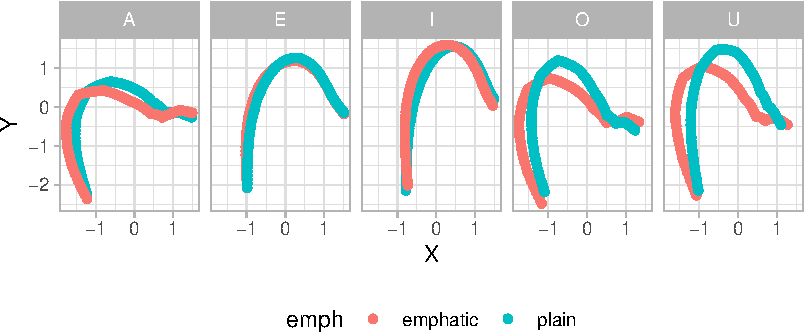
\includegraphics[keepaspectratio]{index_files/figure-pdf/fig-emph-pred-1.pdf}}

}

\caption{\label{fig-emph-pred}}

\end{figure}%

\textsubscript{Source:
\href{https://stefanocoretta.github.io/mv_uti/index.qmd.html}{Article
Notebook}}

\phantomsection\label{cell-fig-emph-ci}
\begin{Shaded}
\begin{Highlighting}[]
\NormalTok{emph\_gam\_p }\SpecialCharTok{|\textgreater{}} 
  \FunctionTok{ggplot}\NormalTok{(}\FunctionTok{aes}\NormalTok{(X, Y, }\AttributeTok{colour =}\NormalTok{ emph)) }\SpecialCharTok{+}
  \FunctionTok{geom\_errorbarh}\NormalTok{(}\FunctionTok{aes}\NormalTok{(}\AttributeTok{xmin =}\NormalTok{ X\_lo, }\AttributeTok{xmax =}\NormalTok{ X\_hi), }\AttributeTok{alpha =} \FloatTok{0.25}\NormalTok{) }\SpecialCharTok{+}
  \FunctionTok{geom\_errorbar}\NormalTok{(}\FunctionTok{aes}\NormalTok{(}\AttributeTok{ymin =}\NormalTok{ Y\_lo, }\AttributeTok{ymax =}\NormalTok{ Y\_hi), }\AttributeTok{alpha =} \FloatTok{0.25}\NormalTok{) }\SpecialCharTok{+}
  \FunctionTok{geom\_point}\NormalTok{(}\AttributeTok{size =} \DecValTok{1}\NormalTok{, }\AttributeTok{alpha =} \FloatTok{0.75}\NormalTok{) }\SpecialCharTok{+}
  \FunctionTok{scale\_color\_brewer}\NormalTok{(}\AttributeTok{type =} \StringTok{"qual"}\NormalTok{, }\AttributeTok{palette =} \StringTok{"Dark2"}\NormalTok{) }\SpecialCharTok{+}
  \FunctionTok{coord\_fixed}\NormalTok{() }\SpecialCharTok{+}
  \FunctionTok{facet\_grid}\NormalTok{(}\AttributeTok{cols =} \FunctionTok{vars}\NormalTok{(vowel)) }\SpecialCharTok{+}
  \FunctionTok{theme\_light}\NormalTok{() }\SpecialCharTok{+}
  \FunctionTok{theme}\NormalTok{(}\AttributeTok{legend.position =} \StringTok{"bottom"}\NormalTok{)}
\end{Highlighting}
\end{Shaded}

\begin{figure}[H]

\centering{

\pandocbounded{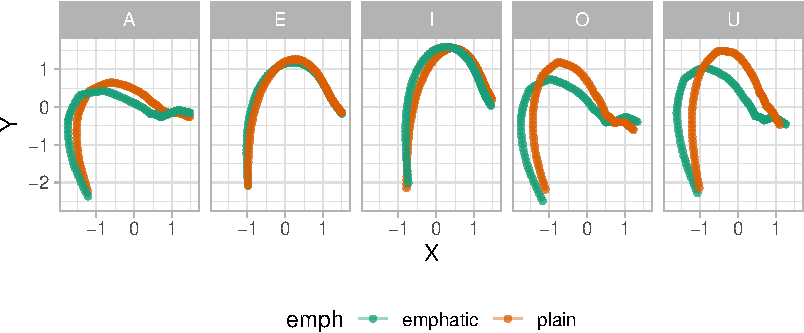
\includegraphics[keepaspectratio]{index_files/figure-pdf/fig-emph-ci-1.pdf}}

}

\caption{\label{fig-emph-ci}}

\end{figure}%

\textsubscript{Source:
\href{https://stefanocoretta.github.io/mv_uti/index.qmd.html}{Article
Notebook}}

\begin{Shaded}
\begin{Highlighting}[]
\NormalTok{emph\_gam\_p\_2 }\OtherTok{\textless{}{-}} \FunctionTok{predict}\NormalTok{(emph\_gam, frame\_emph, }\AttributeTok{se.fit =} \ConstantTok{TRUE}\NormalTok{) }\SpecialCharTok{|\textgreater{}}
  \FunctionTok{as.data.frame}\NormalTok{() }\SpecialCharTok{|\textgreater{}}
  \FunctionTok{as\_tibble}\NormalTok{()}
\FunctionTok{colnames}\NormalTok{(emph\_gam\_p\_2) }\OtherTok{\textless{}{-}} \FunctionTok{c}\NormalTok{(}\StringTok{"X"}\NormalTok{, }\StringTok{"Y"}\NormalTok{, }\StringTok{"X\_se"}\NormalTok{, }\StringTok{"Y\_se"}\NormalTok{)}

\NormalTok{emph\_gam\_p\_2 }\OtherTok{\textless{}{-}} \FunctionTok{bind\_cols}\NormalTok{(frame\_emph, emph\_gam\_p\_2) }\SpecialCharTok{|\textgreater{}}
  \FunctionTok{mutate}\NormalTok{(}
    \AttributeTok{X\_lo =}\NormalTok{ X }\SpecialCharTok{{-}}\NormalTok{ (}\FloatTok{1.96} \SpecialCharTok{*}\NormalTok{ X\_se),}
    \AttributeTok{X\_hi =}\NormalTok{ X }\SpecialCharTok{+}\NormalTok{ (}\FloatTok{1.96} \SpecialCharTok{*}\NormalTok{ X\_se),}
    \AttributeTok{Y\_lo =}\NormalTok{ Y }\SpecialCharTok{{-}}\NormalTok{ (}\FloatTok{1.96} \SpecialCharTok{*}\NormalTok{ Y\_se),}
    \AttributeTok{Y\_hi =}\NormalTok{ Y }\SpecialCharTok{+}\NormalTok{ (}\FloatTok{1.96} \SpecialCharTok{*}\NormalTok{ Y\_se)}
\NormalTok{  ) }\SpecialCharTok{|\textgreater{}} 
  \FunctionTok{separate}\NormalTok{(vow\_emph, }\FunctionTok{c}\NormalTok{(}\StringTok{"vowel"}\NormalTok{, }\StringTok{"emph"}\NormalTok{))}
\end{Highlighting}
\end{Shaded}

\textsubscript{Source:
\href{https://stefanocoretta.github.io/mv_uti/index.qmd.html}{Article
Notebook}}

\phantomsection\label{cell-fig-emph-part}
\begin{Shaded}
\begin{Highlighting}[]
\NormalTok{emph\_gam\_p\_2 }\SpecialCharTok{|\textgreater{}} 
  \FunctionTok{ggplot}\NormalTok{(}\FunctionTok{aes}\NormalTok{(X, Y, }\AttributeTok{colour =}\NormalTok{ emph)) }\SpecialCharTok{+}
  \FunctionTok{geom\_errorbarh}\NormalTok{(}\FunctionTok{aes}\NormalTok{(}\AttributeTok{xmin =}\NormalTok{ X\_lo, }\AttributeTok{xmax =}\NormalTok{ X\_hi), }\AttributeTok{alpha =} \FloatTok{0.5}\NormalTok{) }\SpecialCharTok{+}
  \FunctionTok{geom\_errorbar}\NormalTok{(}\FunctionTok{aes}\NormalTok{(}\AttributeTok{ymin =}\NormalTok{ Y\_lo, }\AttributeTok{ymax =}\NormalTok{ Y\_hi), }\AttributeTok{alpha =} \FloatTok{0.5}\NormalTok{) }\SpecialCharTok{+}
  \CommentTok{\# geom\_point() +}
  \FunctionTok{facet\_grid}\NormalTok{(}\AttributeTok{rows =} \FunctionTok{vars}\NormalTok{(participant), }\AttributeTok{cols =} \FunctionTok{vars}\NormalTok{(vowel)) }\SpecialCharTok{+}
  \FunctionTok{coord\_fixed}\NormalTok{()}
\end{Highlighting}
\end{Shaded}

\begin{figure}[H]

\centering{

\pandocbounded{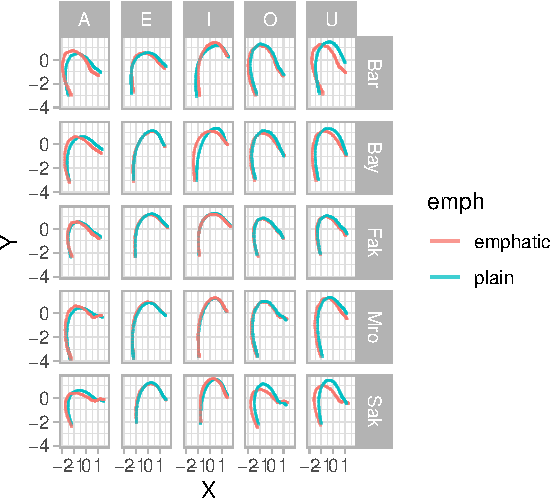
\includegraphics[keepaspectratio]{index_files/figure-pdf/fig-emph-part-1.pdf}}

}

\caption{\label{fig-emph-part}}

\end{figure}%

\textsubscript{Source:
\href{https://stefanocoretta.github.io/mv_uti/index.qmd.html}{Article
Notebook}}

\begin{Shaded}
\begin{Highlighting}[]
\NormalTok{frame\_emph }\OtherTok{\textless{}{-}} \FunctionTok{expand\_grid}\NormalTok{(}
  \AttributeTok{participant =} \FunctionTok{unique}\NormalTok{(dlc\_emph\_f}\SpecialCharTok{$}\NormalTok{participant),}
  \AttributeTok{vow\_emph =} \FunctionTok{unique}\NormalTok{(dlc\_emph\_f}\SpecialCharTok{$}\NormalTok{vow\_emph),}
  \AttributeTok{knot =} \DecValTok{0}\SpecialCharTok{:}\DecValTok{10}
\NormalTok{)}

\NormalTok{pred\_grid\_a }\OtherTok{\textless{}{-}} \FunctionTok{filter}\NormalTok{(}
\NormalTok{  frame\_emph, vow\_emph }\SpecialCharTok{==} \StringTok{"E.plain"}\NormalTok{,}
\NormalTok{  participant }\SpecialCharTok{==} \StringTok{"Sak"}
\NormalTok{)}
\NormalTok{pred\_grid\_b }\OtherTok{\textless{}{-}} \FunctionTok{filter}\NormalTok{(}
\NormalTok{  frame\_emph, vow\_emph }\SpecialCharTok{==} \StringTok{"E.emphatic"}\NormalTok{,}
\NormalTok{  participant }\SpecialCharTok{==} \StringTok{"Sak"}
\NormalTok{)}

\NormalTok{pred\_a }\OtherTok{\textless{}{-}} \FunctionTok{predict.gam}\NormalTok{(emph\_gam, pred\_grid\_a, }\AttributeTok{type =} \StringTok{"lpmatrix"}\NormalTok{) }\SpecialCharTok{|\textgreater{}} 
  \FunctionTok{as\_tibble}\NormalTok{() }\SpecialCharTok{|\textgreater{}} 
  \FunctionTok{mutate}\NormalTok{(}
    \FunctionTok{across}\NormalTok{(}\FunctionTok{starts\_with}\NormalTok{(}\StringTok{"s(knot,participant)"}\NormalTok{), }\SpecialCharTok{\textasciitilde{}}\DecValTok{0}\NormalTok{)}
\NormalTok{  ) }\SpecialCharTok{|\textgreater{}} 
  \FunctionTok{as.matrix}\NormalTok{()}
\CommentTok{\# pred\_a[,301:603] \textless{}{-} 0}
\NormalTok{pred\_a[,}\DecValTok{1}\SpecialCharTok{:}\DecValTok{300}\NormalTok{] }\OtherTok{\textless{}{-}} \DecValTok{0}

\NormalTok{pred\_b }\OtherTok{\textless{}{-}} \FunctionTok{predict.gam}\NormalTok{(emph\_gam, pred\_grid\_b, }\AttributeTok{type =} \StringTok{"lpmatrix"}\NormalTok{) }\SpecialCharTok{|\textgreater{}} 
  \FunctionTok{as\_tibble}\NormalTok{() }\SpecialCharTok{|\textgreater{}} 
  \FunctionTok{mutate}\NormalTok{(}
    \FunctionTok{across}\NormalTok{(}\FunctionTok{starts\_with}\NormalTok{(}\StringTok{"s(knot,participant)"}\NormalTok{), }\SpecialCharTok{\textasciitilde{}}\DecValTok{0}\NormalTok{)}
\NormalTok{  ) }\SpecialCharTok{|\textgreater{}} 
  \FunctionTok{as.matrix}\NormalTok{()}
\CommentTok{\# pred\_b[,301:603] \textless{}{-} 0}
\NormalTok{pred\_b[,}\DecValTok{1}\SpecialCharTok{:}\DecValTok{300}\NormalTok{] }\OtherTok{\textless{}{-}} \DecValTok{0}

\NormalTok{pred\_diff }\OtherTok{\textless{}{-}}\NormalTok{ pred\_a }\SpecialCharTok{{-}}\NormalTok{ pred\_b}
\NormalTok{diff }\OtherTok{\textless{}{-}} \FunctionTok{as.vector}\NormalTok{(pred\_diff }\SpecialCharTok{\%*\%}\NormalTok{ stats}\SpecialCharTok{::}\FunctionTok{coef}\NormalTok{(emph\_gam))}

\NormalTok{se }\OtherTok{\textless{}{-}} \FunctionTok{sqrt}\NormalTok{(}\FunctionTok{rowSums}\NormalTok{((pred\_diff }\SpecialCharTok{\%*\%}\NormalTok{ stats}\SpecialCharTok{::}\FunctionTok{vcov}\NormalTok{(emph\_gam)) }\SpecialCharTok{*}\NormalTok{ pred\_diff))}

\NormalTok{diff\_out }\OtherTok{\textless{}{-}}\NormalTok{ pred\_grid\_a}
\NormalTok{diff\_out}\SpecialCharTok{$}\NormalTok{diff }\OtherTok{\textless{}{-}}\NormalTok{ diff}
\NormalTok{diff\_out}\SpecialCharTok{$}\NormalTok{se }\OtherTok{\textless{}{-}}\NormalTok{ se}
\NormalTok{diff\_out}\SpecialCharTok{$}\NormalTok{lower\_ci }\OtherTok{\textless{}{-}}\NormalTok{ diff }\SpecialCharTok{{-}}\NormalTok{ se }\SpecialCharTok{*} \FloatTok{1.96}
\NormalTok{diff\_out}\SpecialCharTok{$}\NormalTok{upper\_ci }\OtherTok{\textless{}{-}}\NormalTok{ diff }\SpecialCharTok{+}\NormalTok{ se }\SpecialCharTok{*} \FloatTok{1.96}
\end{Highlighting}
\end{Shaded}

\textsubscript{Source:
\href{https://stefanocoretta.github.io/mv_uti/index.qmd.html}{Article
Notebook}}

\begin{Shaded}
\begin{Highlighting}[]
\NormalTok{diff\_out }\SpecialCharTok{|\textgreater{}} 
  \FunctionTok{ggplot}\NormalTok{(}\FunctionTok{aes}\NormalTok{(knot, diff)) }\SpecialCharTok{+}
  \FunctionTok{geom\_hline}\NormalTok{(}\AttributeTok{yintercept =} \DecValTok{0}\NormalTok{) }\SpecialCharTok{+}
  \FunctionTok{geom\_ribbon}\NormalTok{(}\FunctionTok{aes}\NormalTok{(}\AttributeTok{ymin =}\NormalTok{ lower\_ci, }\AttributeTok{ymax =}\NormalTok{ upper\_ci), }\AttributeTok{alpha =} \FloatTok{0.5}\NormalTok{) }\SpecialCharTok{+}
  \FunctionTok{geom\_point}\NormalTok{()}
\end{Highlighting}
\end{Shaded}

\pandocbounded{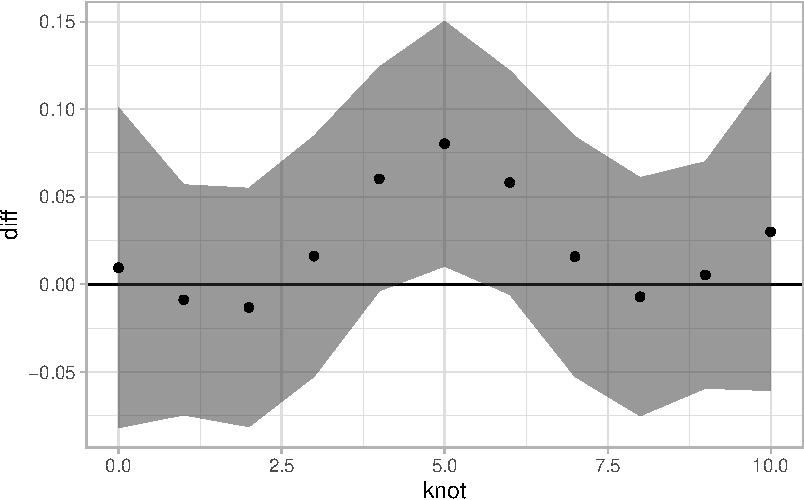
\includegraphics[keepaspectratio]{index_files/figure-pdf/unnamed-chunk-4-1.pdf}}

\textsubscript{Source:
\href{https://stefanocoretta.github.io/mv_uti/index.qmd.html}{Article
Notebook}}

\subsection{FPCA}\label{fpca}

\subsubsection{VC coarticulation}\label{vc-coarticulation-1}

We will apply Multivariate Functional Principal Component Analysis
(MFPCA). The following code has been adapted from Gubian (2024). The
packages below are needed to run MFPCA (except landmarkregUtils, they
are available on CRAN).

\begin{Shaded}
\begin{Highlighting}[]
\FunctionTok{library}\NormalTok{(fda)}
\end{Highlighting}
\end{Shaded}

\begin{verbatim}
Loading required package: splines
\end{verbatim}

\begin{verbatim}
Loading required package: fds
\end{verbatim}

\begin{verbatim}
Loading required package: rainbow
\end{verbatim}

\begin{verbatim}
Loading required package: MASS
\end{verbatim}

\begin{verbatim}

Attaching package: 'MASS'
\end{verbatim}

\begin{verbatim}
The following object is masked from 'package:dplyr':

    select
\end{verbatim}

\begin{verbatim}
Loading required package: pcaPP
\end{verbatim}

\begin{verbatim}
Loading required package: RCurl
\end{verbatim}

\begin{verbatim}

Attaching package: 'RCurl'
\end{verbatim}

\begin{verbatim}
The following object is masked from 'package:tidyr':

    complete
\end{verbatim}

\begin{verbatim}
Loading required package: deSolve
\end{verbatim}

\begin{verbatim}

Attaching package: 'fda'
\end{verbatim}

\begin{verbatim}
The following object is masked from 'package:graphics':

    matplot
\end{verbatim}

\begin{Shaded}
\begin{Highlighting}[]
\FunctionTok{library}\NormalTok{(funData)}
\end{Highlighting}
\end{Shaded}

\begin{verbatim}

Attaching package: 'funData'
\end{verbatim}

\begin{verbatim}
The following object is masked from 'package:ggplot2':

    ggplot
\end{verbatim}

\begin{verbatim}
The following object is masked from 'package:stats':

    integrate
\end{verbatim}

\begin{Shaded}
\begin{Highlighting}[]
\FunctionTok{library}\NormalTok{(MFPCA)}
\CommentTok{\# install.packages("remotes")}
\CommentTok{\# remotes::install\_github("uasolo/landmarkregUtils")}
\FunctionTok{library}\NormalTok{(landmarkregUtils)}
\end{Highlighting}
\end{Shaded}

\textsubscript{Source:
\href{https://stefanocoretta.github.io/mv_uti/index.qmd.html}{Article
Notebook}}

The format required to work through MFPCA is a ``long'' format with one
column containing the coordinate labels (\emph{x} or \emph{y}
coordinate) and another with the coordinate values. We can easily pivot
the data with \texttt{pivot\_longer()}. Note that we are using the
\emph{z}-scored coordinate values (\texttt{X\_z} and \texttt{Y\_z}). If
you are not unsure about what the code in this section, it is always
useful to inspect intermediate and final output.

\begin{Shaded}
\begin{Highlighting}[]
\NormalTok{dlc\_voff\_long }\OtherTok{\textless{}{-}}\NormalTok{ dlc\_voff\_f }\SpecialCharTok{|\textgreater{}} 
  \CommentTok{\# Select relevant columns}
\NormalTok{  dplyr}\SpecialCharTok{::}\FunctionTok{select}\NormalTok{(X\_z, Y\_z, frame\_id, knot, vowel, c2\_place, language, speaker) }\SpecialCharTok{|\textgreater{}} 
  \CommentTok{\# Pivot data to longer format. Saves coordinate labels to column \textasciigrave{}dim\textasciigrave{}}
  \FunctionTok{pivot\_longer}\NormalTok{(}\FunctionTok{c}\NormalTok{(X\_z, Y\_z), }\AttributeTok{names\_to =} \StringTok{"dim"}\NormalTok{)}
\end{Highlighting}
\end{Shaded}

\textsubscript{Source:
\href{https://stefanocoretta.github.io/mv_uti/index.qmd.html}{Article
Notebook}}

In the second step, we create a \texttt{multiFunData} object: this is a
special type of list object, with the observations of the two
coordinates (\texttt{X\_z} and \texttt{Y\_z}) as two matrices of
dimension \(N \cdot 11\), where \(N\) is the number of tongue contours
and \(11\) is for the 11 knots returned by DLC. Three columns in the
data are used to create the \texttt{multiFunData} object: one column
with the id of each contour (in our data, \texttt{frame\_id}), a time or
series column (\texttt{knot}) and the column with the coordinate values
(\texttt{value}).

\begin{Shaded}
\begin{Highlighting}[]
\NormalTok{curves\_fun\_2d }\OtherTok{\textless{}{-}} \FunctionTok{lapply}\NormalTok{(}
  \FunctionTok{c}\NormalTok{(}\StringTok{"X\_z"}\NormalTok{, }\StringTok{"Y\_z"}\NormalTok{),}
  \ControlFlowTok{function}\NormalTok{(y) \{}
    \FunctionTok{long2irregFunData}\NormalTok{(}
\NormalTok{      dlc\_voff\_long }\SpecialCharTok{|\textgreater{}} \FunctionTok{filter}\NormalTok{(dim }\SpecialCharTok{==}\NormalTok{ \{\{y\}\}),}
      \CommentTok{\# Tongue contour ID}
      \AttributeTok{id =} \StringTok{"frame\_id"}\NormalTok{,}
      \CommentTok{\# Knot column}
      \AttributeTok{time =} \StringTok{"knot"}\NormalTok{,}
      \CommentTok{\# X/Y coordinate values}
      \AttributeTok{value =} \StringTok{"value"}
\NormalTok{    ) }\SpecialCharTok{|\textgreater{}} 
    \FunctionTok{as.funData}\NormalTok{()}
\NormalTok{  \}}
\NormalTok{) }\SpecialCharTok{|\textgreater{}} 
  \FunctionTok{multiFunData}\NormalTok{()}
\end{Highlighting}
\end{Shaded}

\textsubscript{Source:
\href{https://stefanocoretta.github.io/mv_uti/index.qmd.html}{Article
Notebook}}

Once we have our \texttt{multFunData} object, we can use the
\texttt{MFPCA()} function to compute an MFPCA. In this tutorial we will
compute the first two PCs, but you can compute up to \(K-1\) PCs where
\(K\) is the number of DLC knots in the data.

\begin{Shaded}
\begin{Highlighting}[]
\CommentTok{\# Number of PC to compute}
\NormalTok{n\_pc }\OtherTok{\textless{}{-}} \DecValTok{2}

\CommentTok{\# Compute MFPCA}
\NormalTok{mfpca }\OtherTok{\textless{}{-}} \FunctionTok{MFPCA}\NormalTok{(}
\NormalTok{  curves\_fun\_2d,}
  \AttributeTok{M =}\NormalTok{ n\_pc,}
  \AttributeTok{uniExpansions =} \FunctionTok{list}\NormalTok{(}\FunctionTok{list}\NormalTok{(}\AttributeTok{type =} \StringTok{"uFPCA"}\NormalTok{), }\FunctionTok{list}\NormalTok{(}\AttributeTok{type =} \StringTok{"uFPCA"}\NormalTok{))}
\NormalTok{)}
\end{Highlighting}
\end{Shaded}

\textsubscript{Source:
\href{https://stefanocoretta.github.io/mv_uti/index.qmd.html}{Article
Notebook}}

We can quickly calculate the proportion of explained variance of each PC
with the following code. PC1 and PC2 together explain almost 100\% of
the variance in our data. The higher the variance explained, the better
the variance patterns in the data are captured.

\begin{Shaded}
\begin{Highlighting}[]
\CommentTok{\# Proportion of explained variance}
\NormalTok{mfpca}\SpecialCharTok{$}\NormalTok{values  }\SpecialCharTok{/} \FunctionTok{sum}\NormalTok{(mfpca}\SpecialCharTok{$}\NormalTok{values)}
\end{Highlighting}
\end{Shaded}

\begin{verbatim}
[1] 0.7108713 0.2891287
\end{verbatim}

\textsubscript{Source:
\href{https://stefanocoretta.github.io/mv_uti/index.qmd.html}{Article
Notebook}}

The best way to assess the effect of the PC scores on the shape of the
tongue contours is to plot the predicted tongue contours based on a set
of representative PC scores. In order to be able to plot the predicted
contours, we need to calculate them from the MFPCA object. Gubian
suggests plotting predicted curves at score intervals based on fractions
of the scores standard deviation. This is what the following code does.

\begin{Shaded}
\begin{Highlighting}[]
\CommentTok{\# Ge the PC score SD}
\NormalTok{sd\_fun }\OtherTok{\textless{}{-}} \FunctionTok{sqrt}\NormalTok{(mfpca}\SpecialCharTok{$}\NormalTok{values)}

\CommentTok{\# PC curves to be plotted}
\NormalTok{pc\_curves }\OtherTok{\textless{}{-}} \FunctionTok{expand\_grid}\NormalTok{(}
  \AttributeTok{PC =} \DecValTok{1}\SpecialCharTok{:}\NormalTok{n\_pc,}
  \AttributeTok{dim =} \DecValTok{1}\SpecialCharTok{:}\DecValTok{2}\NormalTok{,}
  \CommentTok{\# Set the SD fraction, from {-}1 SD to +1 SD, with increments by 0.25}
  \AttributeTok{sd\_frac =} \FunctionTok{seq}\NormalTok{(}\SpecialCharTok{{-}}\DecValTok{1}\NormalTok{, }\DecValTok{1}\NormalTok{, }\AttributeTok{by =} \FloatTok{0.25}\NormalTok{)}
\NormalTok{) }\SpecialCharTok{|\textgreater{}}
  \FunctionTok{group\_by}\NormalTok{(PC, dim, sd\_frac) }\SpecialCharTok{|\textgreater{}}
  \CommentTok{\# We can now calculate the predicted contour with funData2long1().}
  \CommentTok{\# reframe() is needed because the funData2long1() function returns a data frame}
  \CommentTok{\# the has more rows than the original.}
  \FunctionTok{reframe}\NormalTok{(}
    \FunctionTok{funData2long1}\NormalTok{(}
\NormalTok{      mfpca}\SpecialCharTok{$}\NormalTok{meanFunction[[dim]] }\SpecialCharTok{+}
\NormalTok{        sd\_frac }\SpecialCharTok{*}\NormalTok{ sd\_fun[PC] }\SpecialCharTok{*}\NormalTok{ mfpca}\SpecialCharTok{$}\NormalTok{functions[[dim]][PC],}
      \AttributeTok{time =} \StringTok{"knot"}\NormalTok{, }\AttributeTok{value =} \StringTok{"value"}
\NormalTok{    )}
\NormalTok{  ) }\SpecialCharTok{|\textgreater{}} 
  \CommentTok{\# We relabel the dimensions}
  \FunctionTok{mutate}\NormalTok{(}
    \AttributeTok{dim =} \FunctionTok{factor}\NormalTok{(dim, }\AttributeTok{levels =} \FunctionTok{c}\NormalTok{(}\DecValTok{2}\NormalTok{, }\DecValTok{1}\NormalTok{), }\AttributeTok{labels =} \FunctionTok{c}\NormalTok{(}\StringTok{\textquotesingle{}Y\_z\textquotesingle{}}\NormalTok{, }\StringTok{\textquotesingle{}X\_z\textquotesingle{}}\NormalTok{))}
\NormalTok{  )}
\end{Highlighting}
\end{Shaded}

\textsubscript{Source:
\href{https://stefanocoretta.github.io/mv_uti/index.qmd.html}{Article
Notebook}}

The created data frame \texttt{pc\_curves} has the predicted values of
the X and Y coordinates \emph{along the knots}. This is the same
structure as Figure~\ref{fig-tongue-xy}, with the knot number on the
\emph{x}-axis and the coordinates on the \emph{y}-axis. Of course, what
we are after is the X/Y plot of the tongue contours, rather than the
knot/coordinate plot as needed to fit an MFPCA. For the sake of clarity,
we first plot the predicted curves for X and Y separately.
Figure~\ref{fig-pc-curves} shows these. The plot is composed of four
panels: the top two are the predicted curves along knot number for the Y
coordinates (based on PC1 in the left panel and PC2 in the right panel).
Interpreting the effect of the PCs on the X and Y coordinates separately
allows one to observe vertical (Y coordinate) and horizontal (X
coordinate) differences in tongue position independently. However, note
that the vector of muscle contractions in the tongue are not simply
along a vertical/horizontal axis (Honda 1996; A. A. Wrench 2024).
Looking at a full tongue contour (in an X/Y coordinates plot) will
generally prove to be more straightforward.

\phantomsection\label{cell-fig-pc-curves}
\begin{Shaded}
\begin{Highlighting}[]
\NormalTok{pc\_curves }\SpecialCharTok{|\textgreater{}} 
  \FunctionTok{ggplot}\NormalTok{(}\FunctionTok{aes}\NormalTok{(}
    \AttributeTok{x =}\NormalTok{ knot, }\AttributeTok{y =}\NormalTok{ value, }\AttributeTok{group =}\NormalTok{ sd\_frac, }\AttributeTok{color =}\NormalTok{ sd\_frac}
\NormalTok{  )) }\SpecialCharTok{+}
  \FunctionTok{geom\_line}\NormalTok{() }\SpecialCharTok{+}
  \FunctionTok{scale\_color\_gradient2}\NormalTok{(}
    \AttributeTok{low =} \StringTok{"\#762a83"}\NormalTok{, }\AttributeTok{mid =} \StringTok{"grey"}\NormalTok{, }\AttributeTok{high =} \StringTok{"\#1b7837"}\NormalTok{,}
    \AttributeTok{breaks =} \FunctionTok{c}\NormalTok{(}\SpecialCharTok{{-}}\DecValTok{1}\NormalTok{, }\DecValTok{0}\NormalTok{ , }\DecValTok{1}\NormalTok{)}
\NormalTok{  ) }\SpecialCharTok{+}
  \FunctionTok{facet\_grid}\NormalTok{(}
    \AttributeTok{cols =} \FunctionTok{vars}\NormalTok{(PC), }\AttributeTok{rows =} \FunctionTok{vars}\NormalTok{(dim),}
    \AttributeTok{scales =} \StringTok{"free\_y"}\NormalTok{,}
    \AttributeTok{labeller =} \FunctionTok{labeller}\NormalTok{(}\AttributeTok{PC =} \SpecialCharTok{\textasciitilde{}}\FunctionTok{str\_glue}\NormalTok{(}\StringTok{"PC\{.x\}"}\NormalTok{))}
\NormalTok{  ) }\SpecialCharTok{+}
  \FunctionTok{labs}\NormalTok{(}\AttributeTok{color =} \FunctionTok{expression}\NormalTok{(}\FunctionTok{frac}\NormalTok{(s[k], sigma[k]))) }\SpecialCharTok{+}
  \FunctionTok{geom\_line}\NormalTok{(}
    \AttributeTok{data =}\NormalTok{ pc\_curves }\SpecialCharTok{|\textgreater{}} \FunctionTok{filter}\NormalTok{(sd\_frac }\SpecialCharTok{==} \DecValTok{0}\NormalTok{),}
    \AttributeTok{color =} \StringTok{\textquotesingle{}black\textquotesingle{}}\NormalTok{, }\AttributeTok{linewidth =} \FloatTok{1.2}
\NormalTok{  )}
\end{Highlighting}
\end{Shaded}

\begin{figure}[H]

\centering{

\pandocbounded{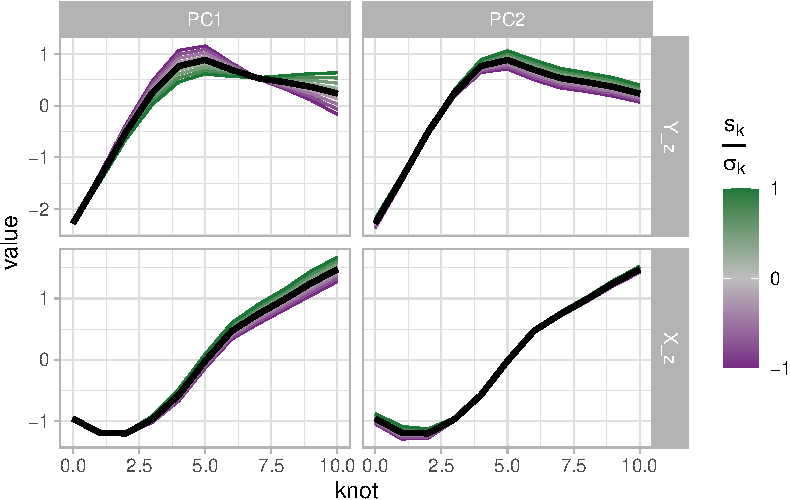
\includegraphics[keepaspectratio]{index_files/figure-pdf/fig-pc-curves-1.pdf}}

}

\caption{\label{fig-pc-curves}Predicted curves along knot number for X
and Y coordinates, as obtained from an MFPCA.}

\end{figure}%

\textsubscript{Source:
\href{https://stefanocoretta.github.io/mv_uti/index.qmd.html}{Article
Notebook}}

In order to plot tongue contours in the X/Y coordinate system, we simply
need to pivot the data to a wider format.

\begin{Shaded}
\begin{Highlighting}[]
\NormalTok{pc\_curves\_wide }\OtherTok{\textless{}{-}}\NormalTok{ pc\_curves }\SpecialCharTok{|\textgreater{}} 
  \FunctionTok{pivot\_wider}\NormalTok{(}\AttributeTok{names\_from =}\NormalTok{ dim)}
\end{Highlighting}
\end{Shaded}

\textsubscript{Source:
\href{https://stefanocoretta.github.io/mv_uti/index.qmd.html}{Article
Notebook}}

Figure~\ref{fig-contours} plots the predicted contours based on the the
PC scores (specifically, fractions of the standard deviation of the PC
scores). The \emph{x} and \emph{y}-axes correspond to the X and Y
coordinates of the tongue contour, with the effect of PC1 in the left
panel and the effect of PC2 in the right panel. A higher PC1 score
(green lines in the left panel) suggest a lowering of the tongue
body/dorsum and raising of the tongue tip. Since the data contains velar
and coronal consonants, we take this to be capturing the velar/coronal
place of articulation effect. A higher PC2 score (green lines in the
right panel) corresponds to an overall higher tongue position.
Considering that the back/central vowels /a, o, u/ are included in this
data set, we take PC2 to be related with the effect of vowel on the
tongue shape at closure onset.

\phantomsection\label{cell-fig-contours}
\begin{Shaded}
\begin{Highlighting}[]
\NormalTok{pc\_curves\_wide }\SpecialCharTok{|\textgreater{}} 
  \FunctionTok{ggplot}\NormalTok{(}\FunctionTok{aes}\NormalTok{(}\AttributeTok{x =}\NormalTok{ X\_z, }\AttributeTok{y =}\NormalTok{ Y\_z, }\AttributeTok{group =}\NormalTok{ sd\_frac, }\AttributeTok{color =}\NormalTok{ sd\_frac)) }\SpecialCharTok{+}
  \FunctionTok{geom\_path}\NormalTok{() }\SpecialCharTok{+}
  \FunctionTok{scale\_color\_gradient2}\NormalTok{(}
    \AttributeTok{low =} \StringTok{"\#762a83"}\NormalTok{, }\AttributeTok{mid =} \StringTok{"grey"}\NormalTok{, }\AttributeTok{high =} \StringTok{"\#1b7837"}\NormalTok{,}
    \AttributeTok{breaks =} \FunctionTok{c}\NormalTok{(}\SpecialCharTok{{-}}\DecValTok{1}\NormalTok{, }\DecValTok{0}\NormalTok{ , }\DecValTok{1}\NormalTok{)}
\NormalTok{  ) }\SpecialCharTok{+}
  \FunctionTok{facet\_wrap}\NormalTok{(}
    \FunctionTok{vars}\NormalTok{(PC),}
    \AttributeTok{labeller =} \FunctionTok{labeller}\NormalTok{(}\AttributeTok{PC =} \SpecialCharTok{\textasciitilde{}}\FunctionTok{str\_glue}\NormalTok{(}\StringTok{"PC\{.x\}"}\NormalTok{))}
\NormalTok{  ) }\SpecialCharTok{+}
  \FunctionTok{coord\_fixed}\NormalTok{()}
\end{Highlighting}
\end{Shaded}

\begin{figure}[H]

\centering{

\pandocbounded{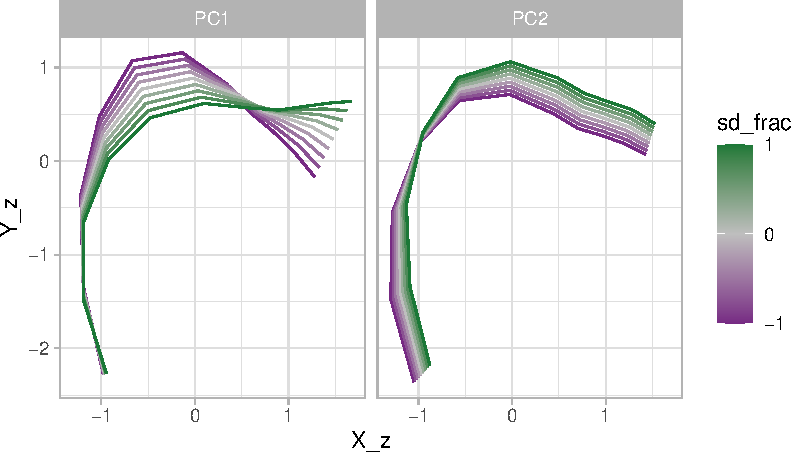
\includegraphics[keepaspectratio]{index_files/figure-pdf/fig-contours-1.pdf}}

}

\caption{\label{fig-contours}Predicted tongue contours as obtained from
an MFPCA.}

\end{figure}%

\textsubscript{Source:
\href{https://stefanocoretta.github.io/mv_uti/index.qmd.html}{Article
Notebook}}

Given the patterns in Figure~\ref{fig-contours}, we can expect to see
differences in PC2 scores based on the vowel if there is VC
coarticulation. We can obtain the PC scores of each observation in the
data with the following code.

\begin{Shaded}
\begin{Highlighting}[]
\NormalTok{pc\_scores }\OtherTok{\textless{}{-}}\NormalTok{ mfpca}\SpecialCharTok{$}\NormalTok{scores }\SpecialCharTok{|\textgreater{}}
  \StringTok{\textasciigrave{}}\AttributeTok{colnames\textless{}{-}}\StringTok{\textasciigrave{}}\NormalTok{(}\FunctionTok{paste0}\NormalTok{(}\StringTok{"PC"}\NormalTok{, }\DecValTok{1}\SpecialCharTok{:}\NormalTok{n\_pc)) }\SpecialCharTok{|\textgreater{}}
  \FunctionTok{as\_tibble}\NormalTok{() }\SpecialCharTok{|\textgreater{}}
  \FunctionTok{bind\_cols}\NormalTok{(dlc\_voff\_long }\SpecialCharTok{|\textgreater{}} \FunctionTok{distinct}\NormalTok{(frame\_id, vowel, c2\_place, language))}
\end{Highlighting}
\end{Shaded}

\textsubscript{Source:
\href{https://stefanocoretta.github.io/mv_uti/index.qmd.html}{Article
Notebook}}

Figure~\ref{fig-pc-scores} plots PC scores by language (rows), consonant
place (columns) and vowel (colour). Both in Italian and Polish, we can
observe a clear coarticulatory effect of /u/ on the production of
coronal stops (and perhaps minor differences in /a/ vs /o/). On the
other hand, the effect of vowel in velar stops seems to be minimal,
again in both languages. This is not entirely surprising, since while
coronal stops allow for adjustments of (and coarticulatory effect on)
the tongue body, velar stops do not since it is precisely the tongue
body/dorsum that is raised to produce the velar closure.

\phantomsection\label{cell-fig-pc-scores}
\begin{Shaded}
\begin{Highlighting}[]
\NormalTok{pc\_scores }\SpecialCharTok{|\textgreater{}} 
  \FunctionTok{filter}\NormalTok{(PC2 }\SpecialCharTok{\textless{}} \FloatTok{0.5}\NormalTok{) }\SpecialCharTok{|\textgreater{}}
  \FunctionTok{ggplot}\NormalTok{(}\FunctionTok{aes}\NormalTok{(}\AttributeTok{x =}\NormalTok{ PC1, }\AttributeTok{y =}\NormalTok{ PC2, }\AttributeTok{color =}\NormalTok{ vowel)) }\SpecialCharTok{+}
  \FunctionTok{geom\_point}\NormalTok{() }\SpecialCharTok{+}
  \FunctionTok{stat\_ellipse}\NormalTok{() }\SpecialCharTok{+}
  \FunctionTok{facet\_grid}\NormalTok{(}\AttributeTok{cols =} \FunctionTok{vars}\NormalTok{(c2\_place), }\AttributeTok{rows =} \FunctionTok{vars}\NormalTok{(language)) }\SpecialCharTok{+}
  \FunctionTok{scale\_color\_brewer}\NormalTok{(}\AttributeTok{palette =} \StringTok{"Dark2"}\NormalTok{)}
\end{Highlighting}
\end{Shaded}

\begin{figure}[H]

\centering{

\pandocbounded{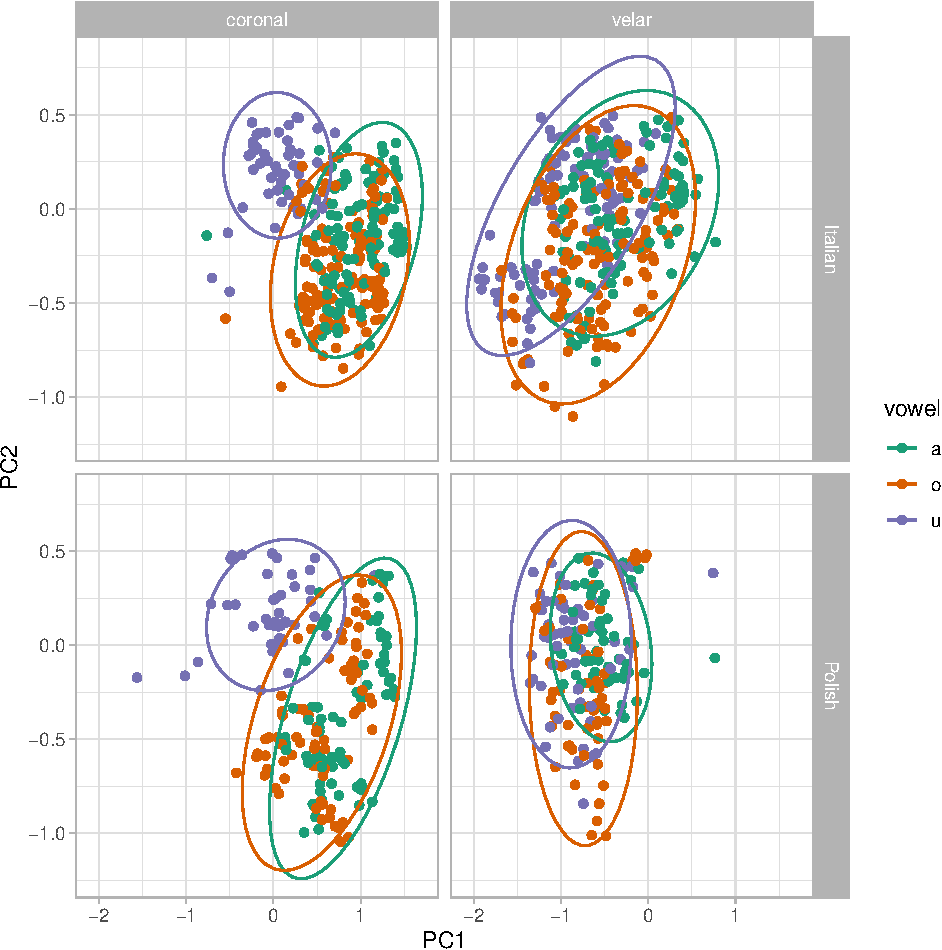
\includegraphics[keepaspectratio]{index_files/figure-pdf/fig-pc-scores-1.pdf}}

}

\caption{\label{fig-pc-scores}PC1/PC2 scores by language, consonant
place of articulation and vowel.}

\end{figure}%

\textsubscript{Source:
\href{https://stefanocoretta.github.io/mv_uti/index.qmd.html}{Article
Notebook}}

Once one has established which patterns each PC is capturing, PC scores
can be submitted to further statistical modelling, like for example
regression models where the PC scores are outcome variables and several
predictors are include to assess possible differences in PC scores.

\subsubsection{Emphaticness}\label{emphaticness-1}

\begin{Shaded}
\begin{Highlighting}[]
\NormalTok{dlc\_emph\_long }\OtherTok{\textless{}{-}}\NormalTok{ dlc\_emph\_f }\SpecialCharTok{|\textgreater{}} 
  \FunctionTok{pivot\_longer}\NormalTok{(}\FunctionTok{c}\NormalTok{(X\_z, Y\_z), }\AttributeTok{names\_to =} \StringTok{"dim"}\NormalTok{) }\SpecialCharTok{|\textgreater{}} 
  \FunctionTok{group\_by}\NormalTok{(dim, participant) }\SpecialCharTok{|\textgreater{}} 
  \FunctionTok{mutate}\NormalTok{(}
    \AttributeTok{value =}\NormalTok{ (value }\SpecialCharTok{{-}} \FunctionTok{mean}\NormalTok{(value)) }\SpecialCharTok{/} \FunctionTok{sd}\NormalTok{(value)}
\NormalTok{  ) }\SpecialCharTok{|\textgreater{}} 
  \FunctionTok{ungroup}\NormalTok{()}
\end{Highlighting}
\end{Shaded}

\textsubscript{Source:
\href{https://stefanocoretta.github.io/mv_uti/index.qmd.html}{Article
Notebook}}

\begin{Shaded}
\begin{Highlighting}[]
\CommentTok{\# build a multiFunData object}
\NormalTok{curves\_fun\_2d }\OtherTok{\textless{}{-}} \FunctionTok{lapply}\NormalTok{(}
  \FunctionTok{c}\NormalTok{(}\StringTok{"X\_z"}\NormalTok{, }\StringTok{"Y\_z"}\NormalTok{),}
  \ControlFlowTok{function}\NormalTok{(y) \{}
    \FunctionTok{long2irregFunData}\NormalTok{(}
\NormalTok{      dlc\_emph\_long }\SpecialCharTok{|\textgreater{}} \FunctionTok{filter}\NormalTok{(dim }\SpecialCharTok{==}\NormalTok{ \{\{y\}\}),}
      \AttributeTok{id =} \StringTok{"frame\_id"}\NormalTok{,}
      \AttributeTok{time =} \StringTok{"knot"}\NormalTok{,}
      \AttributeTok{value =} \StringTok{"value"}
\NormalTok{    ) }\SpecialCharTok{|\textgreater{}} 
    \FunctionTok{as.funData}\NormalTok{()}
\NormalTok{  \}}
\NormalTok{) }\SpecialCharTok{|\textgreater{}} 
  \FunctionTok{multiFunData}\NormalTok{()}
\end{Highlighting}
\end{Shaded}

\textsubscript{Source:
\href{https://stefanocoretta.github.io/mv_uti/index.qmd.html}{Article
Notebook}}

\begin{Shaded}
\begin{Highlighting}[]
\CommentTok{\# Compute FPCA}
\NormalTok{n\_pc }\OtherTok{\textless{}{-}} \DecValTok{2}
\NormalTok{mfpca }\OtherTok{\textless{}{-}} \FunctionTok{MFPCA}\NormalTok{(}
\NormalTok{  curves\_fun\_2d,}
  \AttributeTok{M =}\NormalTok{ n\_pc,}
  \AttributeTok{uniExpansions =} \FunctionTok{list}\NormalTok{(}\FunctionTok{list}\NormalTok{(}\AttributeTok{type =} \StringTok{"uFPCA"}\NormalTok{), }\FunctionTok{list}\NormalTok{(}\AttributeTok{type =} \StringTok{"uFPCA"}\NormalTok{))}
\NormalTok{)}
\end{Highlighting}
\end{Shaded}

\textsubscript{Source:
\href{https://stefanocoretta.github.io/mv_uti/index.qmd.html}{Article
Notebook}}

\begin{Shaded}
\begin{Highlighting}[]
\CommentTok{\# Proportion of explained variance}
\NormalTok{mfpca}\SpecialCharTok{$}\NormalTok{values  }\SpecialCharTok{/} \FunctionTok{sum}\NormalTok{(mfpca}\SpecialCharTok{$}\NormalTok{values)}
\end{Highlighting}
\end{Shaded}

\begin{verbatim}
[1] 0.7309506 0.2690494
\end{verbatim}

\textsubscript{Source:
\href{https://stefanocoretta.github.io/mv_uti/index.qmd.html}{Article
Notebook}}

\begin{Shaded}
\begin{Highlighting}[]
\CommentTok{\# scores st. dev.}
\NormalTok{sd\_fun }\OtherTok{\textless{}{-}} \FunctionTok{sqrt}\NormalTok{(mfpca}\SpecialCharTok{$}\NormalTok{values)}

\CommentTok{\# PC curves to be plotted}
\NormalTok{pc\_curves }\OtherTok{\textless{}{-}} \FunctionTok{expand\_grid}\NormalTok{(}
  \AttributeTok{PC =} \DecValTok{1}\SpecialCharTok{:}\NormalTok{n\_pc,}
  \AttributeTok{dim =} \DecValTok{1}\SpecialCharTok{:}\DecValTok{2}\NormalTok{, }
  \AttributeTok{sd\_frac =} \FunctionTok{seq}\NormalTok{(}\SpecialCharTok{{-}}\DecValTok{1}\NormalTok{, }\DecValTok{1}\NormalTok{, }\AttributeTok{by =} \FloatTok{0.25}\NormalTok{)}
\NormalTok{) }\SpecialCharTok{|\textgreater{}} 
  \FunctionTok{group\_by}\NormalTok{(PC, dim, sd\_frac) }\SpecialCharTok{|\textgreater{}} 
  \FunctionTok{reframe}\NormalTok{(}
    \FunctionTok{funData2long1}\NormalTok{(}
\NormalTok{      mfpca}\SpecialCharTok{$}\NormalTok{meanFunction[[dim]] }\SpecialCharTok{+}
\NormalTok{        sd\_frac }\SpecialCharTok{*}\NormalTok{ sd\_fun[PC] }\SpecialCharTok{*}\NormalTok{ mfpca}\SpecialCharTok{$}\NormalTok{functions[[dim]][PC],}
      \AttributeTok{time =} \StringTok{"knot"}\NormalTok{, }\AttributeTok{value =} \StringTok{"value"}
\NormalTok{    )}
\NormalTok{  ) }\SpecialCharTok{|\textgreater{}} 
  \FunctionTok{mutate}\NormalTok{(}
    \AttributeTok{dim =} \FunctionTok{factor}\NormalTok{(dim, }\AttributeTok{levels =} \FunctionTok{c}\NormalTok{(}\DecValTok{2}\NormalTok{,}\DecValTok{1}\NormalTok{), }\AttributeTok{labels =} \FunctionTok{c}\NormalTok{(}\StringTok{\textquotesingle{}Y\_z\textquotesingle{}}\NormalTok{, }\StringTok{\textquotesingle{}X\_z\textquotesingle{}}\NormalTok{))}
\NormalTok{  )}
\end{Highlighting}
\end{Shaded}

\textsubscript{Source:
\href{https://stefanocoretta.github.io/mv_uti/index.qmd.html}{Article
Notebook}}

\phantomsection\label{cell-fig-emph-pc-curves}
\begin{Shaded}
\begin{Highlighting}[]
\NormalTok{pc\_curves }\SpecialCharTok{|\textgreater{}} 
  \FunctionTok{ggplot}\NormalTok{(}\FunctionTok{aes}\NormalTok{(}
    \AttributeTok{x =}\NormalTok{ knot, }\AttributeTok{y =}\NormalTok{ value, }\AttributeTok{group =}\NormalTok{ sd\_frac, }\AttributeTok{color =}\NormalTok{ sd\_frac}
\NormalTok{  )) }\SpecialCharTok{+}
  \FunctionTok{geom\_line}\NormalTok{() }\SpecialCharTok{+}
  \FunctionTok{scale\_color\_gradient2}\NormalTok{(}
    \AttributeTok{low =} \StringTok{"\#762a83"}\NormalTok{, }\AttributeTok{mid =} \StringTok{"grey"}\NormalTok{, }\AttributeTok{high =} \StringTok{"\#1b7837"}\NormalTok{,}
    \AttributeTok{breaks =} \FunctionTok{c}\NormalTok{(}\SpecialCharTok{{-}}\DecValTok{1}\NormalTok{, }\DecValTok{0}\NormalTok{ , }\DecValTok{1}\NormalTok{)}
\NormalTok{  ) }\SpecialCharTok{+}
  \FunctionTok{facet\_grid}\NormalTok{(}
    \AttributeTok{cols =} \FunctionTok{vars}\NormalTok{(PC), }\AttributeTok{rows =} \FunctionTok{vars}\NormalTok{(dim),}
    \AttributeTok{scales =} \StringTok{"free\_y"}\NormalTok{,}
    \AttributeTok{labeller =} \FunctionTok{labeller}\NormalTok{(}\AttributeTok{PC =} \SpecialCharTok{\textasciitilde{}}\FunctionTok{str\_glue}\NormalTok{(}\StringTok{"PC\{.x\}"}\NormalTok{))}
\NormalTok{  ) }\SpecialCharTok{+}
  \FunctionTok{labs}\NormalTok{(}\AttributeTok{color =} \FunctionTok{expression}\NormalTok{(}\FunctionTok{frac}\NormalTok{(s[k], sigma[k]))) }\SpecialCharTok{+}
  \FunctionTok{geom\_line}\NormalTok{(}
    \AttributeTok{data =}\NormalTok{ pc\_curves }\SpecialCharTok{|\textgreater{}} \FunctionTok{filter}\NormalTok{(sd\_frac }\SpecialCharTok{==} \DecValTok{0}\NormalTok{),}
    \AttributeTok{color =} \StringTok{\textquotesingle{}black\textquotesingle{}}\NormalTok{, }\AttributeTok{linewidth =} \FloatTok{1.2}
\NormalTok{  )}
\end{Highlighting}
\end{Shaded}

\begin{figure}[H]

\centering{

\pandocbounded{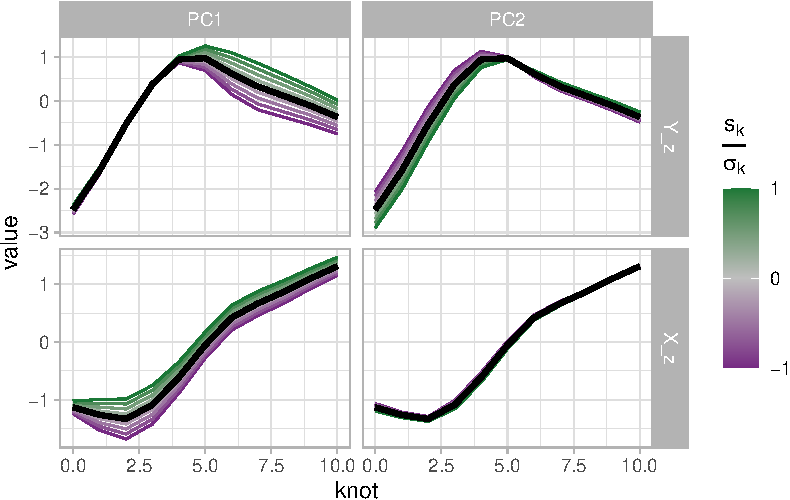
\includegraphics[keepaspectratio]{index_files/figure-pdf/fig-emph-pc-curves-1.pdf}}

}

\caption{\label{fig-emph-pc-curves}}

\end{figure}%

\textsubscript{Source:
\href{https://stefanocoretta.github.io/mv_uti/index.qmd.html}{Article
Notebook}}

\begin{Shaded}
\begin{Highlighting}[]
\NormalTok{pc\_curves\_wide }\OtherTok{\textless{}{-}}\NormalTok{ pc\_curves }\SpecialCharTok{|\textgreater{}} 
  \FunctionTok{pivot\_wider}\NormalTok{(}\AttributeTok{names\_from =}\NormalTok{ dim)}
\end{Highlighting}
\end{Shaded}

\textsubscript{Source:
\href{https://stefanocoretta.github.io/mv_uti/index.qmd.html}{Article
Notebook}}

\phantomsection\label{cell-fig-emph-curves-wide}
\begin{Shaded}
\begin{Highlighting}[]
\NormalTok{pc\_curves\_wide }\SpecialCharTok{|\textgreater{}} 
  \FunctionTok{ggplot}\NormalTok{(}\FunctionTok{aes}\NormalTok{(}\AttributeTok{x =}\NormalTok{ X\_z, }\AttributeTok{y =}\NormalTok{ Y\_z, }\AttributeTok{group =}\NormalTok{ sd\_frac, }\AttributeTok{color =}\NormalTok{ sd\_frac)) }\SpecialCharTok{+}
  \FunctionTok{geom\_path}\NormalTok{() }\SpecialCharTok{+}
  \FunctionTok{scale\_color\_gradient2}\NormalTok{(}
    \AttributeTok{low =} \StringTok{"\#762a83"}\NormalTok{, }\AttributeTok{mid =} \StringTok{"grey"}\NormalTok{, }\AttributeTok{high =} \StringTok{"\#1b7837"}\NormalTok{,}
    \AttributeTok{breaks =} \FunctionTok{c}\NormalTok{(}\SpecialCharTok{{-}}\DecValTok{1}\NormalTok{, }\DecValTok{0}\NormalTok{ , }\DecValTok{1}\NormalTok{)}
\NormalTok{  ) }\SpecialCharTok{+}
  \FunctionTok{facet\_wrap}\NormalTok{(}
    \FunctionTok{vars}\NormalTok{(PC),}
    \AttributeTok{labeller =} \FunctionTok{labeller}\NormalTok{(}\AttributeTok{PC =} \SpecialCharTok{\textasciitilde{}}\FunctionTok{str\_glue}\NormalTok{(}\StringTok{"PC\{.x\}"}\NormalTok{))}
\NormalTok{  ) }\SpecialCharTok{+}
  \FunctionTok{coord\_fixed}\NormalTok{()}
\end{Highlighting}
\end{Shaded}

\begin{figure}[H]

\centering{

\pandocbounded{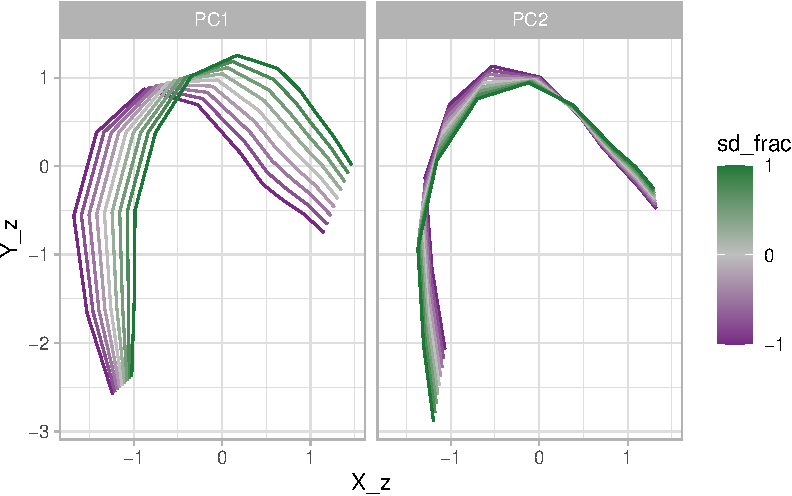
\includegraphics[keepaspectratio]{index_files/figure-pdf/fig-emph-curves-wide-1.pdf}}

}

\caption{\label{fig-emph-curves-wide}}

\end{figure}%

\textsubscript{Source:
\href{https://stefanocoretta.github.io/mv_uti/index.qmd.html}{Article
Notebook}}

\begin{Shaded}
\begin{Highlighting}[]
\CommentTok{\# collect PC scores}
\NormalTok{pc\_scores }\OtherTok{\textless{}{-}}\NormalTok{ mfpca}\SpecialCharTok{$}\NormalTok{scores }\SpecialCharTok{|\textgreater{}}
  \StringTok{\textasciigrave{}}\AttributeTok{colnames\textless{}{-}}\StringTok{\textasciigrave{}}\NormalTok{( }\FunctionTok{paste0}\NormalTok{(}\StringTok{"PC"}\NormalTok{, }\DecValTok{1}\SpecialCharTok{:}\NormalTok{n\_pc)) }\SpecialCharTok{|\textgreater{}}
  \FunctionTok{as\_tibble}\NormalTok{() }\SpecialCharTok{|\textgreater{}}
  \FunctionTok{bind\_cols}\NormalTok{(dlc\_emph\_long }\SpecialCharTok{|\textgreater{}} \FunctionTok{distinct}\NormalTok{(frame\_id, emph, vowel, participant))}
\end{Highlighting}
\end{Shaded}

\textsubscript{Source:
\href{https://stefanocoretta.github.io/mv_uti/index.qmd.html}{Article
Notebook}}

\phantomsection\label{cell-fig-emph-speakers}
\begin{Shaded}
\begin{Highlighting}[]
\NormalTok{pc\_scores }\SpecialCharTok{|\textgreater{}} 
  \FunctionTok{ggplot}\NormalTok{(}\FunctionTok{aes}\NormalTok{(}\AttributeTok{x =}\NormalTok{ PC1, }\AttributeTok{y =}\NormalTok{ PC2, }\AttributeTok{colour =}\NormalTok{ emph, }\AttributeTok{label =}\NormalTok{ vowel)) }\SpecialCharTok{+}
  \FunctionTok{geom\_point}\NormalTok{(}\AttributeTok{alpha =} \FloatTok{0.5}\NormalTok{) }\SpecialCharTok{+}
  \FunctionTok{scale\_color\_brewer}\NormalTok{(}\AttributeTok{palette =} \StringTok{"Dark2"}\NormalTok{) }\SpecialCharTok{+}
  \FunctionTok{stat\_ellipse}\NormalTok{() }\SpecialCharTok{+}
  \FunctionTok{facet\_grid}\NormalTok{(}\AttributeTok{cols =} \FunctionTok{vars}\NormalTok{(participant), }\AttributeTok{rows =} \FunctionTok{vars}\NormalTok{(vowel))}
\end{Highlighting}
\end{Shaded}

\begin{figure}[H]

\centering{

\pandocbounded{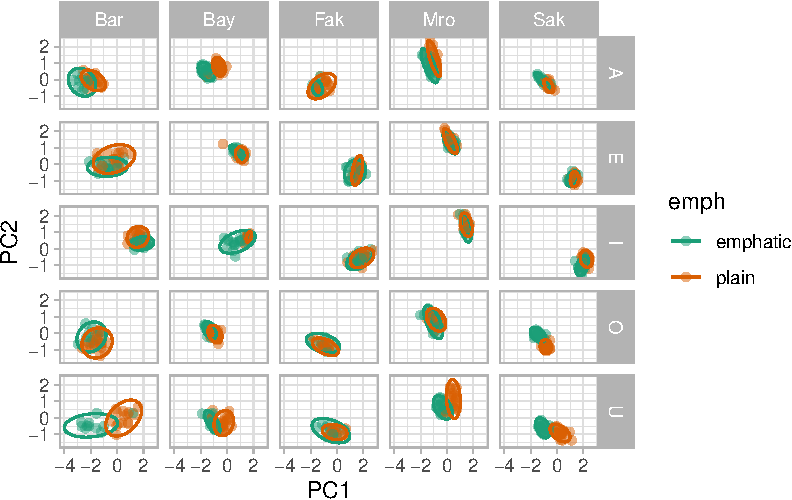
\includegraphics[keepaspectratio]{index_files/figure-pdf/fig-emph-speakers-1.pdf}}

}

\caption{\label{fig-emph-speakers}}

\end{figure}%

\textsubscript{Source:
\href{https://stefanocoretta.github.io/mv_uti/index.qmd.html}{Article
Notebook}}

\phantomsection\label{cell-fig-emph-pc1}
\begin{Shaded}
\begin{Highlighting}[]
\NormalTok{pc\_scores }\SpecialCharTok{|\textgreater{}} 
  \FunctionTok{ggplot}\NormalTok{(}\FunctionTok{aes}\NormalTok{(vowel, PC1, }\AttributeTok{colour =}\NormalTok{ emph)) }\SpecialCharTok{+}
  \FunctionTok{geom\_jitter}\NormalTok{(}\AttributeTok{position =} \FunctionTok{position\_jitterdodge}\NormalTok{(}\AttributeTok{jitter.width =} \FloatTok{0.2}\NormalTok{), }\AttributeTok{alpha =} \FloatTok{0.25}\NormalTok{) }\SpecialCharTok{+}
  \FunctionTok{scale\_color\_brewer}\NormalTok{(}\AttributeTok{palette =} \StringTok{"Dark2"}\NormalTok{) }\SpecialCharTok{+}
    \FunctionTok{facet\_wrap}\NormalTok{(}\FunctionTok{vars}\NormalTok{(participant))}
\end{Highlighting}
\end{Shaded}

\begin{figure}[H]

\centering{

\pandocbounded{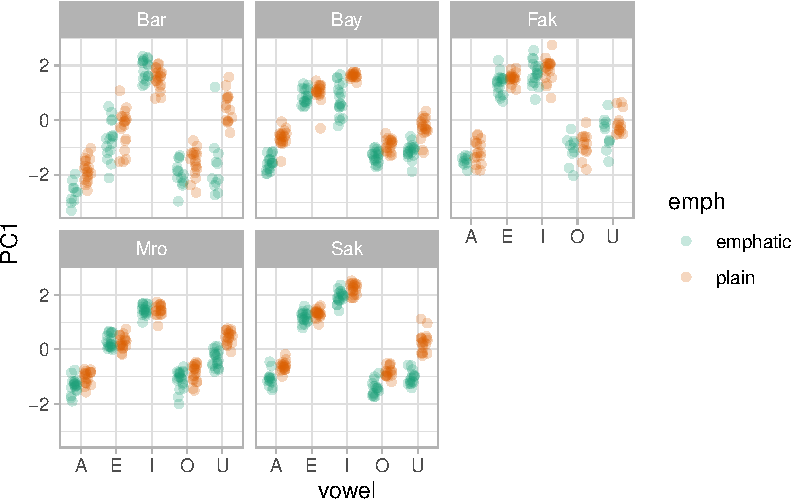
\includegraphics[keepaspectratio]{index_files/figure-pdf/fig-emph-pc1-1.pdf}}

}

\caption{\label{fig-emph-pc1}}

\end{figure}%

\textsubscript{Source:
\href{https://stefanocoretta.github.io/mv_uti/index.qmd.html}{Article
Notebook}}

\phantomsection\label{cell-fig-emph-pc2}
\begin{Shaded}
\begin{Highlighting}[]
\NormalTok{pc\_scores }\SpecialCharTok{|\textgreater{}} 
  \FunctionTok{ggplot}\NormalTok{(}\FunctionTok{aes}\NormalTok{(vowel, PC2, }\AttributeTok{colour =}\NormalTok{ emph)) }\SpecialCharTok{+}
  \FunctionTok{geom\_jitter}\NormalTok{(}\AttributeTok{position =} \FunctionTok{position\_jitterdodge}\NormalTok{(}\AttributeTok{jitter.width =} \FloatTok{0.2}\NormalTok{), }\AttributeTok{alpha =} \FloatTok{0.25}\NormalTok{) }\SpecialCharTok{+}
  \FunctionTok{scale\_color\_brewer}\NormalTok{(}\AttributeTok{palette =} \StringTok{"Dark2"}\NormalTok{) }\SpecialCharTok{+}
    \FunctionTok{facet\_wrap}\NormalTok{(}\FunctionTok{vars}\NormalTok{(participant))}
\end{Highlighting}
\end{Shaded}

\begin{figure}[H]

\centering{

\pandocbounded{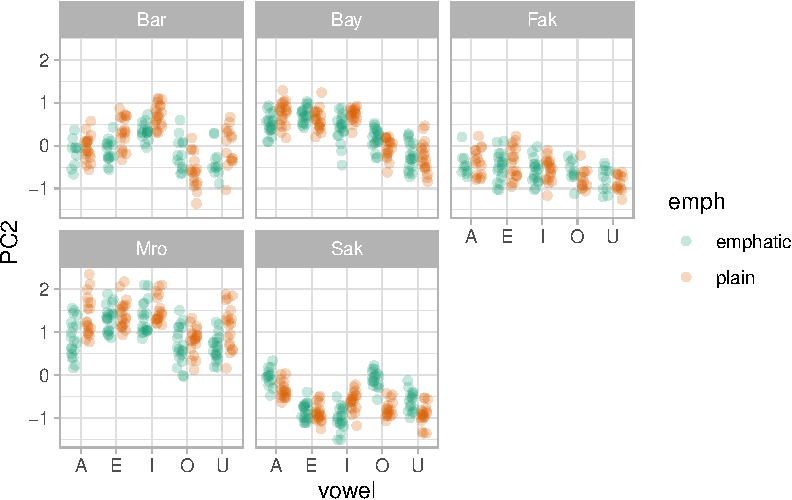
\includegraphics[keepaspectratio]{index_files/figure-pdf/fig-emph-pc2-1.pdf}}

}

\caption{\label{fig-emph-pc2}}

\end{figure}%

\textsubscript{Source:
\href{https://stefanocoretta.github.io/mv_uti/index.qmd.html}{Article
Notebook}}

\phantomsection\label{refs}
\begin{CSLReferences}{1}{0}
\bibitem[\citeproctext]{ref-coretta2018f}
Coretta, Stefano. 2018. {``An Exploratory Study of the Voicing Effect in
Italian and Polish {[}Data V1.0.0{]}.''}
\url{https://doi.org/10.17605/OSF.IO/8ZHKU}.

\bibitem[\citeproctext]{ref-coretta2020}
---------. 2020a. {``Longer Vowel Duration Correlates with Greater
Tongue Root Advancement at Vowel Offset: Acoustic and Articulatory Data
from Italian and Polish.''} \emph{The Journal of the Acoustical Society
of America} 147: 245259. \url{https://doi.org/10.1121/10.0000556}.

\bibitem[\citeproctext]{ref-coretta2020b}
---------. 2020b. {``Vowel Duration and Consonant Voicing: A Production
Study.''} PhD thesis.

\bibitem[\citeproctext]{ref-gubian2024}
Gubian, Michele. 2024. \emph{Workshop on Functional PCA for Phonetics
and Prosody}. \url{https://github.com/uasolo/FPCA-phonetics-workshop}.

\bibitem[\citeproctext]{ref-hastie1986}
Hastie, Trevor, and Robert Tibshirani. 1986. {``Generalized Additive
Models.''} \emph{Statistical Science} 1 (3): 297310.
\url{https://doi.org/10.1201/9780203753781-6}.

\bibitem[\citeproctext]{ref-honda1996}
Honda, Kiyoshi. 1996. {``Organization of Tongue Articulation for
Vowels.''} \emph{Journal of Phonetics} 24 (1): 3952.
\url{https://doi.org/10.1006/jpho.1996.0004}.

\bibitem[\citeproctext]{ref-pedersen2019}
Pedersen, Eric J., David L. Miller, Gavin L. Simpson, and Noam Ross.
2019. {``Hierarchical Generalized Additive Models in Ecology: An
Introduction with Mgcv.''} \emph{PeerJ} 7: e6876.
\url{https://doi.org/10.7717/peerj.6876}.

\bibitem[\citeproctext]{ref-soskuthy2021}
Sóskuthy, Márton. 2021a. {``Evaluating Generalised Additive Mixed
Modelling Strategies for Dynamic Speech Analysis.''} \emph{Journal of
Phonetics} 84: 101017. \url{https://doi.org/10.1016/j.wocn.2020.101017}.

\bibitem[\citeproctext]{ref-soskuthy2017a}
---------. 2021b. {``Generalised Additive Mixed Models for Dynamic
Analysis in Linguistics: A Practical Introduction.''}
\url{https://doi.org/10.48550/arXiv.1703.05339}.

\bibitem[\citeproctext]{ref-wieling2018}
Wieling, Martijn. 2018. {``Analyzing Dynamic Phonetic Data Using
Generalized Additive Mixed Modeling: A Tutorial Focusing on Articulatory
Differences Between L1 and L2 Speakers of English.''} \emph{Journal of
Phonetics} 70: 86116. \url{https://doi.org/10.1016/j.wocn.2018.03.002}.

\bibitem[\citeproctext]{ref-wood2006}
Wood, Simon. 2006. \emph{Generalized Additive Models: An Introduction
with r}. CRC Press.

\bibitem[\citeproctext]{ref-wrench2024}
Wrench, Alan A. 2024. {``The Compartmental Tongue.''} \emph{Journal of
Speech, Language, and Hearing Research} 67 (10S): 38873913.
\url{https://doi.org/10.1044/2024_jslhr-23-00125}.

\bibitem[\citeproctext]{ref-wrench2022}
Wrench, Alan, and Jonathan Balch-Tomes. 2022. {``Beyond the Edge:
Markerless Pose Estimation of Speech Articulators from Ultrasound and
Camera Images Using DeepLabCut.''} \emph{Sensors} 22 (3): 1133.
\url{https://doi.org/10.3390/s22031133}.

\end{CSLReferences}




\end{document}
